\chapter{\IfLanguageName{dutch}{Methodologie}{Methodology}}
\label{ch:methodologie}

Om te onderzoeken welke types modellen best presteren zal er voor elke combinatie van seizoensgebonden of niet-seizoensgebonden en univariate of multivariate data een notebook opgesteld worden. Op het einde van elke notebook zal dan aan elk model een foutscore toegekend zijn. Deze foutscore wordt bepaald door het gemiddelde te nemen van de mean average errors van elke partitie bij de datasetverdeling door cross-validation. Het model met de laagste foutscore zal de meest accurate voorspelling gemaakt hebben bij het type invoerdata bij dit deelprobleem voor de gebruikte data. 

Er dient echter vermeld te worden dat dit in zekere mate altijd zal afhangen van de invoerdata en dit type model niet noodzakelijk de beste prestatie zal leveren bij dit type invoerdata.

\section{Voorbereiding}
%\subsection{Benutte libraries}
\subsection{Datavoorbereiding}
\subsubsection{Dataset 1, temperatuur}
Hier zal het het deel van de dataset die de temperatuur weergeeft geformateerd worden  naar een dataset met 1 kolom en een index waarin de maand en het jaartal weergegeven worden van het jaar 1979 tot 2018.

\clearpage
\captionof{listing}{Datavoorbereiding dataset temperatuur}
\label{code:prep_temp}
\begin{minted}[
frame=lines,
framesep=2mm,
fontsize=\footnotesize,
linenos,breaklines
]{python}
# Source: https://www.kaggle.com/rainbowgirl/climate-data-toronto-19372018
tt = pd.read_csv('./data/Toronto_temp.csv')
tt = tt[tt['Day'] == 1]
tt['Year'] = tt['Year'].replace({'2,013':'2013',
'2,014':'2014',
'2,015':'2015',
'2,016':'2016',
'2,017':'2017',
'2,018':'2018'})
# tt.groupby('Year').count()
tt = tt[(tt['Year'] != '1937')]
ttt = tt.groupby('Year').count()
#ttt.head(50)
#tt.groupby('Year').count().tail(50)
meantt = tt.groupby('Year').mean()['Mean Temp (C)']
#meantt.index
#meantt
meantt.sort_index(inplace=True)

plt.xlabel('Years')
plt.ylabel('Temperature (C)')
plt.xticks(np.array(range(0,meantt.size,10)))
plt.scatter(meantt.index, meantt)

print('start : ' + meantt.index[0])
print('end : ' + meantt.index[-1])

new_row = pd.Series({'Mean Temp (C)' : 0.555556, 'Year': '2018', 'Month':12})
tt = tt.append(new_row, ignore_index=True)
tt['Year'] = tt['Year'].astype(int)
mean_temp_monthly = tt[['Year','Month','Mean Temp (C)']].set_index(['Year','Month']).sort_index()
# mean_temp_monthly
mean_temp_monthly = mean_temp_monthly[mean_temp_monthly.index.get_level_values(0).astype(int) >= 1979 ]
mean_temp_monthly
\end{minted}

Op listing \ref{code:prep_temp} wordt de code weergegeven de die ruwe dataset zal omzetten naar een dataset die bruikbaar zal zijn om te gebruiken voor deze bachelorproef. 


De delen die in commentaar staan geven een tussentijdse weergave van de dataset, maar worden niet telkens weergegeven om het aantal tabellen binnen deze sectie overzichtelijk te houden. \\


Zo wordt op lijn 2 het originele csv-bestand ingelezen deze ruwe data zal er uit zien als deze zichtbaar op figuur \ref{fig:tempdatagraph}. \\
Op lijn 3 worden enkel de waarden van de eerste dag van de maand behouden in de dataset \\
Daarna worden van lijn 4 tot lijn 9 de jaartallen aangepast zodat deze overeenkomen met de rest van de dataset. \\
Op lijn 10 wordt het aantal rijen per jaar weergegeven. \\
Op lijn 11 zal het eerste jaar uit de dataset verwijderd worden aangezien deze data onvolledig is. \\
Op lijn 12 wordt het aantal jaren toegekend aan de variabele $ttt$ \\
Op lijn 15 wordt het gemiddelde van de temperaturen van de eerste dagen van de maand per jaar berekend. \\
Op lijn 18 wordt dit gemiddelde gesorteerd. \\



\begin{figure}
    \centering
    \caption{Ruwe invoerdata}
    \label{fig:tempdataraw.png}
    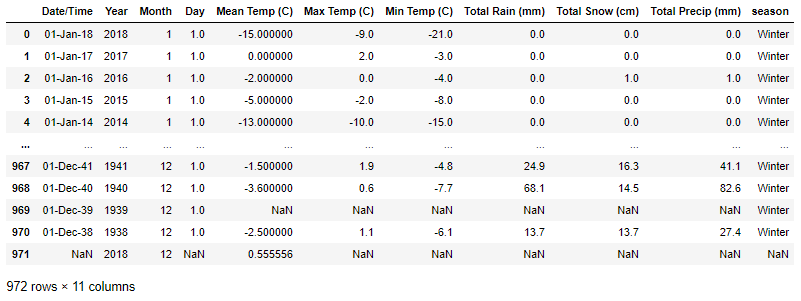
\includegraphics[width=1\linewidth]{temp_data_rawpng}
\end{figure}


Van lijn 20 tot lijn 23 worden de labels en ijkingen gedefini\"{e}erd van de grafiek die de data zal weergeven en zichtbaar is op figuur \ref{fig:tempdatagraph} die op lijn 24 getekend zal worden. \\



\begin{figure}
    \caption{Grafische weergave jaarlijkse temperatuur}
    \label{fig:tempdatagraph}
    \centering
    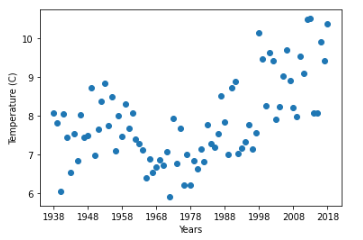
\includegraphics[width=0.7\linewidth]{temp_data_graph}
\end{figure}

Op lijn 25 en 26 worden de start en de eindjaren van deze dataset afgeprint om ze te kunnen vergelijken met de start en de eindjaren van de andere dataset.

Op lijn 28 wordt de laatste waarde voor het jaar 2018 toegevoegd aangezien deze nog niet in de dataset zat. \\
Op lijn 29 wordt deze nieuwe waarde toegevoegd.\\

Op lijn 30 wordt de waarde voor het jaar geconverteerd naar een integer. \\
Op lijn 31 wordt de dataset geindexeerd op jaar en maand. \\
Op lijn 33 worden de jaren die voor 1979 komen uit de dataset gefilterd omdat de waarden voor de andere dataset starten vanaf 1979.\\
Op lijn 34 wordt het resultaat van de dataformattering uitgevoerd zichtbaar op figuur \ref{fig:tempdata}.




\begin{figure}
    \centering
    \caption{Resultaat van data formatting}
    \label{fig:tempdata}
    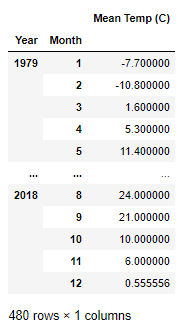
\includegraphics[width=0.3\linewidth]{temp_data}
\end{figure}



\clearpage



\subsubsection{Dataset 2, ijsdikte}

Hier zal het deel van de dataset die de ijsdikte weergeeft geformateerd worden naar een dataset met 1 kolom en het jaartal van het jaar 1979 tot 2018 als index zal dienen.

\captionof{listing}{Datavoorbereiding dataset temperatuur}
\label{code:prep_ice}
\begin{minted}[
frame=lines,
framesep=2mm,
fontsize=\footnotesize,
linenos,breaklines
]{python}
#source: https://nsidc.org/arcticseaicenews/sea-ice-tools/
ice2 = pd.read_csv('./data/seaice2.csv')
# ice2
ice2_mean = ice2.mean()[1:-2]
# ice2_mean
ice2_mean.index = ice2_mean.index.values.astype(int)

plt.title('Yearly ice extent')
plt.scatter(ice2_mean.index,ice2_mean)
plt.xlabel('Years')
plt.ylabel('Extent')
plt.show()

# ice2['2018']
# pd.concat([ice2['2016'],ice2['2017'],ice2['2018'],ice2['2019']]).reset_index()[0]
# ice2[['2018']].append(ice2[['2019']])
ice2.rename(columns={'Unnamed: 0' : 'Month', 'Unnamed: 1' : 'Day'}, inplace = True)
ice2.drop([' ','1981-2010','Day','1978','2020'],axis=1,inplace=True)
values = ice2.values
i = 0
for row in values :
    if type(row[0]) != str :
        values[i][0] = month
    else:
        month = row[0]
    i = i +1
# ice2.columns.values
ice2_clean = pd.DataFrame(values)
ice2_clean.columns = ice2.columns.values
# ice2_clean.head(5)
ice2_monthly_mean = ice2_clean.set_index('Month').astype(float).groupby('Month',sort=False).mean()
# ice2_monthly_mean
# ice2_monthly_mean.T.stack().index.get_level_values(0)
# ice2_monthly_mean.T.stack().reset_index(level=['Month']).drop(columns=['Month'])
ice2_monthly_mean_chron = ice2_monthly_mean.T.stack().reset_index(level=['Month']).drop(columns=['Month'])
# ice2.columns.size
plt.title('Monthly ice extent')
plt.plot(ice2_monthly_mean_chron.values)
plt.xticks(np.array(range(0,500,75)))
plt.xlabel('Cumulative month')
plt.ylabel('Extent')
plt.show()

# np.unique(ice2_monthly_mean_chron.index.values).size*12
print('from ' + ice2_monthly_mean_chron.index.values[0] + ' until ' + ice2_monthly_mean_chron.index.values[-1])
ice2_monthly_mean_chron = ice2_monthly_mean.T.stack().reset_index(level=['Month']).drop(columns=['Month'])
ice2_monthly_mean_chron.columns = ['ice_extent']
ice2_monthly_mean_chron
\end{minted}

Op lijn 2 zal de ijsdataset ingelezen worden en zal er uitzien zoals zichtbaar op figuur \ref{fig:icedataraw} \\
Op lijn 4 zal het gemiddelde genomen worden van alle kolommen tussen eerste en de voorlaatste. De eerste, de voorlaatste en de laatste kolom worden uit de dataset gelaten omdat deze irrelevant zijn voor dit onderzoek. \\
Op lijn 6 worden de indexwaarden geconverteerd naar integers. \\

\begin{figure}
    \centering
    \caption{Ruwe data van de jaarlijkse ijsdiktes}
    \label{fig:icedataraw}
    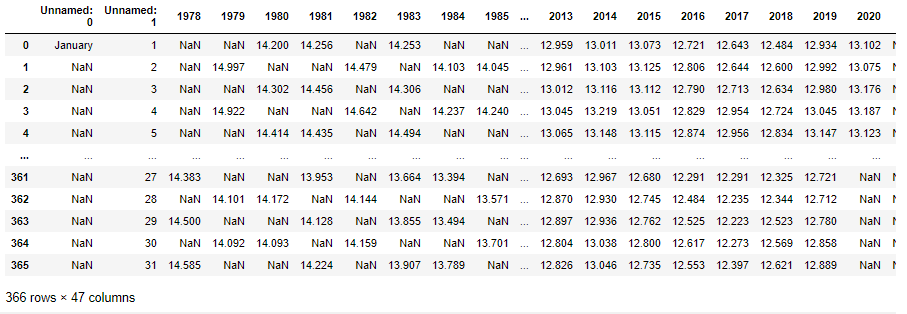
\includegraphics[width=1\linewidth]{ice_data_rawpng}
\end{figure}

De code van lijn 8 tot lijn 12 zal ervoor zorgen dat de jaarlijkse data grafisch weergegeven wordt. \\
Op lijn 17 zullen de kolomnamen hernoemd worden en op lijn 18 worden de overbodige kolommen verwijderd. \\

De code van lijn 18 tot lijn 26 zal er voor zorgen dat de maandkolom aangevuld wordt omdat deze tot hiertoe nog onvolledig zal zijn. \\
Op lijn 28 wordt een nieuwe dataframe ge\"{i}nitialiseerd waarvan de kolommen op lijn 29 aangevuld worden. \\
Op lijn 31 wordt hier het maandelijks gemiddelde genomen van deze nieuwe dataframe en opgeslaan in de variabele en op lijn 35 worden deze in chronologische volgorde geplaatst.\\

Het deel code van lijn 37 tot en met lijn 42 zal zorgen voor de grafische weergave van de maandelijkse ijsdikte weergegeven op figuur\ref{fig:iceextentmonthly}. \\

\begin{figure}
    \centering
    \caption{Grafische weergave van de maandelijkse ijsdiktes}
    \label{fig:iceextentmonthly}
    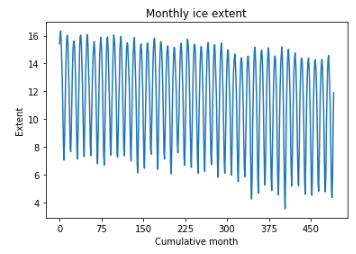
\includegraphics[width=0.7\linewidth]{ice_extent_monthly}
\end{figure}

Op lijn 45 worden de start en eindjaartallen uitgeprint. \\
De code op lijn 46 zal ervoor zorgen dat de maandindex verwijderd wordt.\\
Op lijn 47 zal de kolom hernoemd worden en op lijn 48 zal het resultaat uitgeprint worden, dit zal er uit zien zoals zichtbaar op figuur\ref{fig:iceextentdata}.

\begin{figure}
    \centering
    \caption{Data van de maandelijks ijsdiktes}
    \label{fig:iceextentdata}
    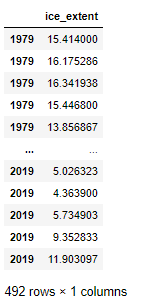
\includegraphics[width=0.3\linewidth]{ice_extent_data}
\end{figure}

\subsubsection{Combineren van de datasets}

In dit deel van de datavoorbereiding zullen de datasets gecombineerd worden.

\captionof{listing}{Datavoorbereiding dataset temperatuur}
\begin{minted}[
frame=lines,
framesep=2mm,
fontsize=\footnotesize,
linenos,breaklines
]{python}
ice2_monthly_mean_chron_cut = ice2_monthly_mean_chron[:-12]
# ice2_monthly_mean_chron
# ice2_monthly_mean_chron_cut
# mean_temp_monthly
# ice2_monthly_mean_chron_cut
combined = mean_temp_monthly[mean_temp_monthly.index.get_level_values(0) >= 1979]
combined['ice_extent'] = ice2_monthly_mean_chron_cut.values
# combined
combined.rename(columns={'Mean Temp (C)': 'mean_temp'}, inplace=True)
dataframe_monthly = combined
# dataframe_monthly
# dataframe_monthly[['mean_temp']]
plt.plot(dataframe_monthly[['mean_temp']].values[-24:],label='temperature')
plt.plot(dataframe_monthly[['ice_extent']].values[-24:],label='ice extent')
plt.legend()
plt.show()
dataframe_yearly = combined.groupby('Year').mean()
# dataframe_yearly
# dataframe_monthly[['mean_temp']].values
plt.plot(dataframe_monthly[['mean_temp']].values,label='temperature')
plt.plot(dataframe_monthly[['ice_extent']].values,label='ice extent')
plt.legend()
dataframe_monthly.to_csv('./data/dataframe_monthly.csv')
dataframe_yearly.to_csv('./data/dataframe_yearly.csv')
\end{minted}

Op lijn 1 worden de laatste 12 waarden van de gemiddelde maandelijkse chronologische dataset in een nieuwe variabele gestoken. \\
Op lijn 6 wordt een nieuwe dataset ge\"{i}nitialiseerd waar de maandelijkse gemiddelde temperaturen van 1979 ingevoerd worden.\\
Op lijn 7 worden de ijsdiktes hieraan toegevoegd. \\
Op lijn 9 wordt de kolom hernoemd op de lijn erna wordt de dataset nog eens toegevoegd aan een duidelijkere variabelenaam. \\

De code op lijn 13 tot 17 zorgt voor de grafische weergave van de gecombineerde dataset van de laatste 2 jaren weergegeven op figuur\ref{fig:combinedlastyears}. Hier valt op te merken dat de ijsdikte zal vergroten wanneer de temperatuur laag is. Dit is logisch aangezien het ijs zal smelten bij hogere temperaturen. \\

\begin{figure}
    \centering
    \caption{Grafische weergave van de ijsdikte en de temperatuur van de laatste 2 jaar}
    \label{fig:combinedlastyears}
    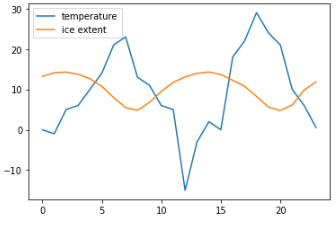
\includegraphics[width=0.7\linewidth]{combined_last_years.PNG}
\end{figure}

De code op lijn 17 zal het jaarlijks gemiddelde nemen.

Op lijn 20 tot 23 wordt de code weergegeven die ervoor zal zorgen dat het volledige maandelijks gemiddelde weergegeven zal worden van 1979 tot 2018. Dit valt te beschouwen op figuur \ref{fig:combinedlastyears}. Hierop kan vastgesteld worden dat de temperatuur lichtjes zal dalen terwijl de ijsdikte zal stijgen.

\begin{figure}
    \centering
    \caption{Grafische weergave van de ijsdikte en de temperatuur}
    \label{fig:combinedmonths}
    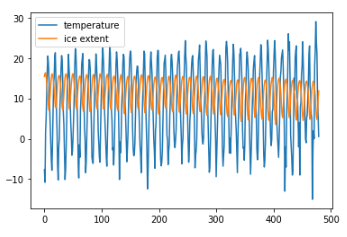
\includegraphics[width=0.7\linewidth]{combined_months.PNG}
\end{figure}

Op lijn 23 en 24 worden de dataframes weggeschreven naar csv-bestanden zodat ze kunnen gebruikt worden bij het opstellen van de modellen.


\section{Univariate niet-seizoensgebonden}

In dit deel zullen de voorspellingsmodellen voor univariate niet-seizoensgebonden data opgesteld worden. De modeltypes die bekeken zullen worden zijn ARIMA, LSTM en Prophet. Om dit te onderzoeken zullen er voorspellingen gemaakt worden van de gemiddelde jaarlijkse temperatuur.

\subsection{Algemene methodes}

Hier worden enkele algemene methodes gedefinieerd namelijk de full\textunderscore graph methode die een grafiek zal weergeven van de ingevoerde gedifferentieerde tijdreeks die ook als invoerparameter gebruikt zal worden samen met de grafiektitel.

Daarnaast wordt ook nog de methode revert\textunderscore diff gedefinieerd waar de gediferentieerde voorspellingen terug omgezet worden naar voorspellingen in miljoenen vierkante kilometers. Hiervoor zijn de gedifferentieerde voorspellingen en de originele dataset nodig als invoerparameters.

\captionof{listing}{Opstellen van algemene methodes}
\begin{minted}[
frame=lines,
framesep=2mm,
fontsize=\footnotesize,
linenos,breaklines
]{python}

# define functions used troughout the notebook

# define function for plotting last prediction and the actual data
def full_graph(predicted_diff, title):

# format predictions by adding NaN values in front
predictionsArray = np.asarray(revert_diff(predicted_diff, ts))
zerosArray = np.zeros(ts.values.size-len(predictionsArray.flatten()))
cleanPrediction = pd.Series(np.concatenate((zerosArray,predictionsArray))).replace(0,np.NaN)
cleanPrediction.index = ts.index.values

# plot
plt.title(title)
plt.plot(ts, marker='o', color='blue',label='Actual values')
plt.plot(cleanPrediction, marker='o', color='red',label='Last 4 year prediction')
plt.ylim([0,15])
plt.legend()

plt.show()

# define function for reverting a differenced dataset
def revert_diff(predicted_diff, og_data):

# retrieve last value
last_value = og_data.iloc[-predicted_diff.size-1][0]

# initialize reverted array
predicted_actual = np.array([])

# add each value in the differenced array with the last actual value
for value_diff in predicted_diff:
actual_value = last_value + value_diff
predicted_actual = np.append(predicted_actual, actual_value)
last_value = actual_value

return predicted_actual
\end{minted}

\subsection{Stationariteit}

Dan zal nagegaan worden in hoeverre deze dataset stationair is met gebruik van de hieronder omschreven test\textunderscore stationarity methode. Dit is noodzakelijk voor het opstellen van het ARIMA model.

\captionof{listing}{Test stationarity}
\begin{minted}[
frame=lines,
framesep=2mm,
fontsize=\footnotesize,
linenos,breaklines
]{python}
# define method to visualise the stationarity of a time series
def test_stationarity(timeseries):

    #Determing rolling statistics
    rolmean = timeseries.rolling(12).mean()
    rolstd = timeseries.rolling(12).std()
    
    #Plot rolling statistics:
    orig = plt.plot(timeseries, color='blue',label='Original')
    mean = plt.plot(rolmean, color='red', label='Rolling Mean')
    std = plt.plot(rolstd, color='black', label = 'Rolling Std')
    plt.legend(loc='best')
    plt.title('Rolling Mean & Standard Deviation')
    plt.show(block=False)

# check stationarity of time serie
test_stationarity(ts)
\end{minted}

Het resultaat van de test\textunderscore stationarity methode wordt weergegeven op figuur \ref{fig:stationarityunivariatenonseasonal}. Daar kan opgemerkt worden dat de data niet stationair is maar er een dalende trend aanwezig is.

\begin{figure}
    \centering
    \caption{Resultaat test stationarity}
    \label{fig:stationarityunivariatenonseasonal}
    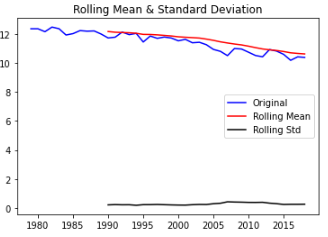
\includegraphics[width=0.7\linewidth]{stationarity_univariate_non_seasonal}
\end{figure}

Om deze trend te neutraliseren en de data stationair te maken zal het random walk difference genomen worden en nogmaals de stationariteit testen.

\captionof{listing}{Test stationarity bij random walk differencing}
\begin{minted}[
frame=lines,
framesep=2mm,
fontsize=\footnotesize,
linenos,breaklines
]{python}
# take the random walk difference of the time serie
ts_diff = ts - ts.shift(1)
ts_diff = ts_diff.dropna()

# display stationarity of the newly differenced time serie
test_stationarity(ts_diff)
\end{minted}

Door hiervan nogmaals de stationariteit te testen wordt figuur\ref{fig:stationarityunivariatenonseasonal2} bekomen. Hierop valt af te lezen dat de data nu wel stationair is.

\begin{figure}
    \centering
    \caption{Resultaat test stationarity na random walk differencing}
    \label{fig:stationarityunivariatenonseasonal2}
    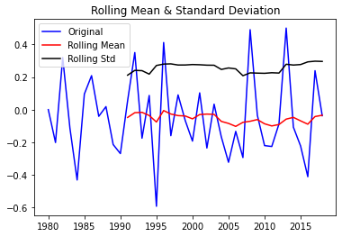
\includegraphics[width=0.7\linewidth]{stationarity_univariate_non_seasonal2}
\end{figure}

\subsection{Cross validation}

Om aan cross validation te doen moet de tijdreeks opgesplitst worden in verschillende reeksen waarbij de testset van de vorige reeks telkens toegevoegd wordt aan de trainingsset van de huidige reeks. Bij de univariate niet-seizoensgebonden tijdreeks wordt telkens een testgrootte van 4 genomen. De waarden worden ook enkel uitgeprint indien de testset groter is dan 20 om een minimale testset te garanderen. De grootte van de train-en testset zal ook geprint worden bij het uitvoeren van dit stuk code.

\captionof{listing}{Code voor het opstellen van cross-validation}
\begin{minted}[
frame=lines,
framesep=2mm,
fontsize=\footnotesize,
linenos,breaklines
]{python}
# initialize TimeSeriesSplit object
tscv = TimeSeriesSplit(n_splits = 8)

# loop trough all split time series that have a trainingsset with more than 20 values
for train_index, test_index in tscv.split(ts_diff):
    if train_index.size > 20:

        # initialize cross validation train and test sets
        cv_train, cv_test = ts_diff.iloc[train_index], ts_diff.iloc[test_index]
        
        # visiualize cross_validation structure for reference
        print("TRAIN:", train_index.size)
        print("TEST:", test_index.size)
        print()
\end{minted}

\subsection{ARIMA}

In dit stuk code worden de hyperparameters bepaald die de beste resultaten zullen behalen. Zo worden alle mogelijke parametercombinaties binnen het ARIMA model getest op de data met cross validation. De best presterende parameters die dus zorgen voor de laagste MAE score worden behouden en zullen gebruikt worden voor de finale voorspelling.

\captionof{listing}{Bepalen van de hyperparameters}
\begin{minted}[
frame=lines,
framesep=2mm,
fontsize=\footnotesize,
linenos,breaklines
]{python}
%%time
# ARIMA
from statsmodels.tsa.arima_model import ARIMA
import itertools
import warnings
import sys
from sklearn.metrics import mean_absolute_error

# Define the p, d and q parameters to take any value between 0 and 2
p = q = range(0, 5)
d = range(0,3)

# Generate all different combinations of p, q and q triplets
pdq = list(itertools.product(p, d, q))

# initialize variables
best_pdq = pdq
best_mean_mae = np.inf

# specify to ignore warning messages to reduce visual clutter
warnings.filterwarnings("ignore") 

# loop trough all possible parameter combinations of pdq
for param in pdq:
    print(param)
    
    # some parametercombinations might lead to crash, so catch exceptions and continue
    try:  
        
        # initialize the array which will contain the mean average errors
        maes = []
        
        # loop trough all split time series that have a trainingsset with more than 20 values
        for train_index, test_index in tscv.split(ts_diff):
            if train_index.size > 20:
            
                # initialize cross validation train and test sets
                cv_train, cv_test = ts_diff.iloc[train_index], ts_diff.iloc[test_index]
                
                # build model
                model = ARIMA(cv_train, order=(param))
                
                # fit model
                model_fit = model.fit()
                
                # make predictions
                predictions =  model_fit.predict(start=len(cv_train), end=len(cv_train)+cv_test.size-1, dynamic=False)
                
                # renaming for clarity
                prediction_values = predictions.values
                true_values = cv_test.values
                
                # error calculation this part of the cross validation
                maes.append(mean_absolute_error(true_values, prediction_values))
            
        
        # error calculation for this parameter combination
        mean_mae = np.mean(maes)
        print('MAE: ' + str(mean_mae))    
        
        # store parameters resulting in the lowest mean MAE
        if mean_mae < best_mean_mae:
            best_mean_mae = mean_mae
            best_maes = maes
            best_pdq = param
            best_predictions = prediction_values
            
    except Exception as e:
    print(e)
    continue

# logging
print()
print('Best MAE = ' + str(best_mean_mae))
print(best_pdq)
\end{minted}

Hieruit blijkt dat de beste parametercombinatie voor een bereik van 0 tot 5 voor de $p$ en $q$ waarden en 0 tot 2 voor de $d$ waarden (3,0,0) zijn. De $d$ waarden blijven zo beperkt omdat een waarde hoger dan 1 in praktijk niet voorkomt zoals beschreven in de literatuurstudie. Dit zijn dan ook de parameterwaarden die gebruikt zullen worden voor de finale iteratie van ARIMA. Een hoger bereik zou tot een beter resultaat kunnen leiden maar ook tot overfitting en zal zeker zorgen voor een hogere uitvoeringstijd omwille van deze redenen is het bereik van $p$ en $q$ beperkt tot 5.

\captionof{listing}{Finale iteratie ARIMA}
\begin{minted}[
frame=lines,
framesep=2mm,
fontsize=\footnotesize,
linenos,breaklines
]{python}
start_time = timeit.default_timer()

# specify to ignore warning messages
warnings.filterwarnings("ignore") 

print("----")

# initialize the array which will contain the mean average errors
maes = []

# loop trough all split time series that have a trainingsset with more than 20 values
for train_index, test_index in tscv.split(ts_diff):
    if train_index.size > 20:
    
        # initialize cross validation train and test sets
        cv_train, cv_test = ts_diff.iloc[train_index], ts_diff.iloc[test_index]
        
        # build model
        arima = ARIMA(cv_train, best_pdq).fit(start_ar_lags=1,disp=False)
        
        # make predictions
        predictions = arima.forecast(steps=4)
        prediction_values = predictions[0]
        true_values = cv_test.values
        
        # error calc
        maes.append(mean_absolute_error(true_values, prediction_values))
        
        # last actual prediction 
        last_prediction_ARIMA = prediction_values
        
        print("I",end="")

# store results to variables
time_ARIMA = timeit.default_timer() - start_time
mae_mean = np.mean(maes)
MAE_ARIMA = mae_mean
last_MAE_ARIMA = maes[-1]

# logging
print()
print('Mean MAE: %.3f x 1 000 000 km\u00b2' % MAE_ARIMA)
print('MAE of last prediction: %.3f x 1 000 000 km\u00b2' % last_MAE_ARIMA)
print('Execution time: %.3f seconds' % time_ARIMA)
full_graph(last_prediction_ARIMA, 'Last prediction ARIMA')
print('Mean average errors:')
print(maes)
\end{minted}

De bovenstaande code zal leiden tot de uitvoer die zichtbaar is op figuur\ref{fig:uvnsarima}. Hier wordt de gemiddelde MAE overheen de verschillende iteraties bij cross validation weergeven alsook de MAE van de laatste voorspelling. Daarnaast wordt ook de uitvoeringstijd weergegeven en ook de voorspelde waarden van de laatste partitie van de cross validation ten opzichte van de originele waarden. Ook de reeks met de MAEs wordt weergegeven.

\begin{figure}
    \centering
    \caption{Resultaat finale iteratie ARIMA}
    \label{fig:uvnsarima}
    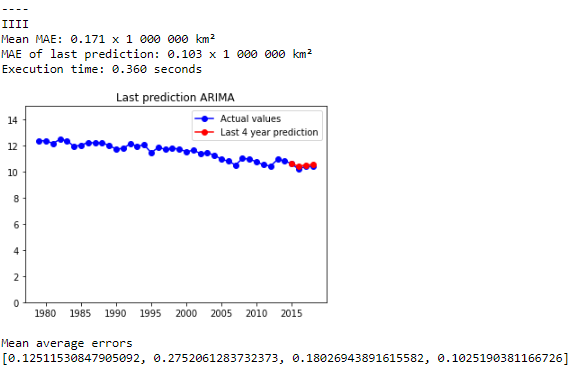
\includegraphics[width=1\linewidth]{uv_ns_ARIMA}
\end{figure}

\clearpage
\subsection{LSTM}

Het volgende model dat getest zal worden is een LSTM model. Aangezien dit een neuraal netwerk is zijn er op voorhand enkele methodes gedefinieerd om het overzicht te bewaren. 

De eerste methode die gedefinieerd wordt is de split\textunderscore sequence dit zal er voor zorgen dat de univariabele tijdreeks opgesplitst wordt in samples zodat deze gebruikt kunnen worden als invoerwaarden voor een LSTM netwerk. De originele tijdreeks dient ingegeven te worden bij sequence, het aantal invoerstappen en het aantal uitvoerstappen dienen ook meegegeven te worden.

Daarnaast wordt ook de methode build\textunderscore model gedefinieerd die het model zal opstellen. Dit zal gebeuren door de structuur van het LSTM model op te stellen met gebruik van het aantal features, het aantal neuronen in de LSTM laag, de dropout rate en de batchgrootte deze parameters diennen ook ingegeven te worden. Na het opstellen van het model zal het gefit worden aan de trainingsdata.

Ten slotte wordt ook nog de functie predict opgesteld. Deze functie verwacht de trainingsset, het model en het aantal features als invoerwaarde en zal het verdere verloop van de tijdreeks trachten te voorspellen. 

\captionof{listing}{Functies voor het opstellen van een LSTM model}
\begin{minted}[
frame=lines,
framesep=2mm,
fontsize=\footnotesize,
linenos,breaklines
]{python}
from keras.layers import Dropout
# split a univariate sequence into samples
def split_sequence(sequence, n_steps_in, n_steps_out):
    X, y = list(), list()
    for i in range(len(sequence)):
        # find the end of this pattern
        end_ix = i + n_steps_in
        out_end_ix = end_ix + n_steps_out
        
        # check if we are beyond the sequence
        if out_end_ix > len(sequence):
        break
        
        # gather input and output parts of the pattern
        seq_x, seq_y = sequence[i:end_ix], sequence[end_ix:out_end_ix]
        X.append(seq_x)
        y.append(seq_y)
    return array(X), array(y)

def build_model(raw_seq, n_steps_in, n_steps_out, n_features, n_neurons, dropout, batch_s):

    # split into samples
    X, y = split_sequence(raw_seq.values.flatten(), n_steps_in, n_steps_out)
    
    # reshape from [samples, timesteps] into [samples, timesteps, features]
    X = X.reshape((X.shape[0], X.shape[1], n_features))
    
    # define model
    model = Sequential()
    model.add(LSTM(n_neurons, activation='relu'))
    model.add(Dropout(dropout))
    model.add(Dense(n_steps_out))
    model.compile(optimizer='adam', loss='mae')
    
    # fit model
    model.fit(X, y, batch_size=batch_s, epochs=100, verbose=0)
    
    return model


def predict(x_input, model, n_features):
    n_features = 1
    
    # reshape data
    x_input = x_input.reshape((1, n_steps_in, n_features))
    
    # predict
    yhat = model.predict(x_input, verbose=0)
    
    return yhat
\end{minted}

Ook bij LSTM dienen de hyperparameters geoptimaliseerd te worden. Dit gebeurt door middel van onderstaande code. Waarbij een reeks mogelijk waarden gedefinieerd wordt op lijn 15 tot 18 waarvan alle mogelijk combinaties getest worden en waarvan de best presterende combinatie bijgehouden wordt.

\captionof{listing}{Bepalen van de hyperparameters}
\begin{minted}[
frame=lines,
framesep=2mm,
fontsize=\footnotesize,
linenos,breaklines
]{python}
%%time

# Disabled tf warning because of visual clutter
tf.compat.v1.logging.set_verbosity(tf.compat.v1.logging.ERROR)


# constant variables
n_steps_in = 4
n_steps_out = 4
n_features  = 1
maes = []
global_maes = []

# optimizable variables
n_neurons_array = [1,10,20]
dropout_array = [0,0.5,0.99]
batch_size_array = [1,8]


# initialize values
best_MAE = 100
best_n_neurons = 0
best_activation = 'none'
best_dropout = 0
best_batch_size = 0

# loop over all possible parameter combinations
for n_neurons in n_neurons_array:
    for dropout in dropout_array:
        for batch_size in batch_size_array:
        
            print("----")
            
            # loop trough all split time series that have a trainingsset with more than 20 values
            for train_index, test_index in tscv.split(ts_diff): 
                if train_index.size > 20:  
                
                    # initialize cross validation train and test sets
                    y_train, y_test = ts_diff.iloc[train_index], ts_diff.iloc[test_index]
                    
                    # build model
                    lstm_model = build_model(y_train, n_steps_in, n_steps_out, n_features, n_neurons, dropout, batch_size)
                    
                    # make predictions
                    x_input = array(y_test)
                    y_predicted = predict(x_input, lstm_model, n_features).flatten()
                    y_actual = y_test.values
                    
                    # error calculation this part of the cross validation
                    maes.append(mean_absolute_error(y_actual, y_predicted))
                    
                    print("I",end="")
                    
                    # last actual prediction 
                    last_prediction_LSTM = y_predicted
                    
            # error calculation for this parameter combination
            MAE_LSTM = np.mean(maes)
            last_MAE_LSTM = maes[-1]
            global_maes.append(MAE_LSTM)
            
            # store parameters resulting in the lowest mean MAE
            if best_MAE > MAE_LSTM:
                best_n_neurons = n_neurons
                best_dropout = dropout
                best_batch_size = batch_size
                best_MAE = MAE_LSTM
            
            # log values for parameter combination
            print()
            print(n_neurons)
            print(dropout)
            print(batch_size)
            print(MAE_LSTM)
            print()    

# log parameter combination with best result
print('Best:')
print('N neurons')
print(best_n_neurons)
print('Dropout rate')
print(best_dropout)
print('Batch size')
print(best_batch_size)
print('MAE')
print(best_MAE)
plt.bar(range(0,len(global_maes)), global_maes)
\end{minted}

Na het uitvoeren van deze code blijkt er nauwelijks verschil te zijn bij het aanpassen van de hyperparameters. Dit valt af te leiden uit de MAE's die weergegeven worden door de plot op lijn 87. Die figuur\ref{fig:uvnslstmbar} als resultaat zal hebben.
Dit blijkt ook wanneer deze code meerdere malen doorlopen wordt aangezien er verschillende resultaten bekomen worden.

\begin{figure}
    \centering
    \caption{Grafische weergave verschil in MAE's bij verschillende hyperparameters met MAE op de y-as}
    \label{fig:uvnslstmbar}
    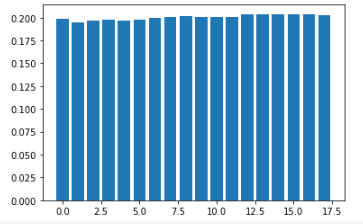
\includegraphics[width=1\linewidth]{uv_ns_LSTM_bar}
\end{figure}

Om verder te gaan zullen de waarden 1 voor het aantal neuronen gebruikt worden, 0 voor de beste dropout rate en 8 voor de batch size. 

\captionof{listing}{Finale iteratie LSTM}
\begin{minted}[
frame=lines,
framesep=2mm,
fontsize=\footnotesize,
linenos,breaklines
]{python}

%%time

start_time = timeit.default_timer()

# Disabled tf warning because of visual clutter
tf.compat.v1.logging.set_verbosity(tf.compat.v1.logging.ERROR)


# constant variables
n_steps_in = 4
n_steps_out = 4
n_features  = 1
maes = []


# optimizable variables
n_neurons = best_n_neurons
dropout = best_dropout
batch_s = best_batch_s

print("----")

# loop trough all split time series that have a trainingsset with more than 20 values
for train_index, test_index in tscv.split(ts_diff):
    if train_index.size > 20:  
        # initialize cross validation train and test sets
        y_train, y_test = ts_diff.iloc[train_index], ts_diff.iloc[test_index]
        
        # build model
        lstm_model = build_model(y_train, n_steps_in, n_steps_out, n_features, n_neurons, dropout, batch_s)
        
        # make predictions
        x_input = array(y_test)
        y_predicted = predict(x_input, lstm_model, n_features).flatten()
        y_actual = y_test.values
        
        # error calc
        maes.append(mean_absolute_error(y_actual, y_predicted))
        
        print("I",end="")
    
# last actual prediction 
last_prediction_LSTM = y_predicted

# store variables
time_LSTM = timeit.default_timer() - start_time
MAE_LSTM = np.mean(maes)
last_MAE_LSTM = maes[-1]

# visualisation
print()
print('Mean MAE: %.3f x 1 000 000 km\u00b2' % MAE_LSTM)
print('MAE of last prediction: %.3f x 1 000 000 km\u00b2' % last_MAE_LSTM)
print('Execution time: %.3f seconds' % time_LSTM)
full_graph(last_prediction_LSTM, 'Last prediction LSTM')
print('Mean average errors')
print(maes)
\end{minted}

De bovenstaande code zal leiden tot de uitvoer die zichtbaar is op figuur\ref{fig:uvns}. Ook hier kan de gemiddelde MAE overheen de verschillende iteraties bij cross validation weergeven worden alsook de MAE van de laatste voorspelling. Daarnaast wordt ook de uitvoeringstijd weergegeven en ook de voorspelde waarden van de laatste partitie van de cross validation ten opzichte van de originele waarden. Ook de reeks met de MAEs wordt weergegeven. Net zoals bij ARIMA.

\begin{figure}
    \centering
    \caption{Resultaat finale iteratie LSTM}
    \label{fig:uvnslstm}
    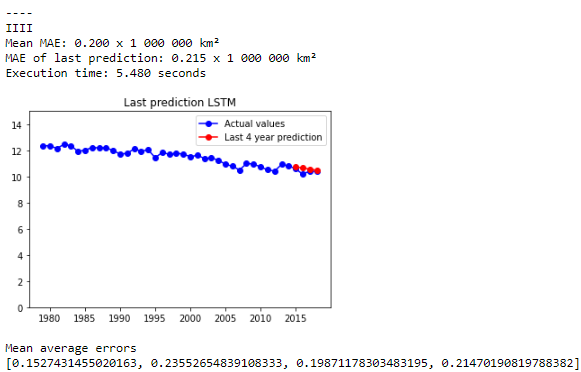
\includegraphics[width=1\linewidth]{uv_ns_LSTM}
\end{figure}

\clearpage
\subsection{Prophet}

Als laatste dient ook Prophet nog bekeken te worden voor het voorspellen van de tijdreeks. Hier zal eerst de data opnieuw geformateerd moeten worden aangezien prophet een bepaalde structuur hantereert.

\captionof{listing}{Code voor het formatteren van de data voor Prophet}
\begin{minted}[
frame=lines,
framesep=2mm,
fontsize=\footnotesize,
linenos,breaklines
]{python}
# formatting dataframe
ts_formated_prophet = ts_diff.reset_index().rename(columns = {'Year' : 'ds', 'ice_extent' : 'y'})
ts_formated_prophet['ds'] = pd.DataFrame(pd.to_datetime(ts_formated_prophet['ds'].astype(str), format='%Y'))
\end{minted}

Daarna kan de hyperparameter voor changepoint\textunderscore prior\textunderscore scale die zal staan voor de frequentie van het aanduiden changepoints (punten waar de data van een trend zal afwijken) bepaald worden met behulp van onderstaande code.

\captionof{listing}{Code voor het bepalen van de hyperparameters}
\begin{minted}[
frame=lines,
framesep=2mm,
fontsize=\footnotesize,
linenos,breaklines
]{python}

# Python
import itertools
import numpy as np
import pandas as pd

# define dataframe
df = ts_formated_prophet

param_grid = {  
'changepoint_prior_scale': [0.001, 0.01, 0.1, 1, 2, 5, 10, 15, 20, 25],
}

# Generate all combinations of parameters
all_params = [dict(zip(param_grid.keys(), v)) for v in itertools.product(*param_grid.values())]

# initialize variables
maes = []  
global_maes = []
best_MAE_prophet = np.inf

# Use cross validation to evaluate all parameters
for params in all_params:

    # loop trough all split time series that have a trainingsset with more than 20 values
    for train_index, test_index in tscv.split(ts_formated_prophet):    
        if train_index.size > 20:  
        
            # initialize cross validation train and test sets
            train  = ts_formated_prophet.iloc[train_index]
            y_test = ts_formated_prophet.iloc[test_index][['y']].values.flatten()
            X_test = ts_formated_prophet.iloc[test_index][['ds']]
            
            # Fit model with given params
            model = Prophet(**params, weekly_seasonality=False, daily_seasonality=False)
            model = model.fit(train)
            
            # make predictions
            forecast = model.predict(X_test)
            y_pred = forecast['yhat'].values
            
            # last actual prediction 
            last_prediction_prophet = y_pred
            
            # error calculation this part of the cross validation
            maes.append(mean_absolute_error(y_test, y_pred))
    
    # error calculation for this parameter combination
    MAE_prophet = np.mean(maes)
    last_MAE_prophet = maes[-1]
    global_maes.append(MAE_prophet)
    
    # logging
    print('changepoint_prior_scale: ' + str(params['changepoint_prior_scale']))
    
    # store parameters resulting in the lowest mean MAE
    if best_MAE_prophet > MAE_prophet:
    best_params = params
    best_MAE_prophet = MAE_prophet

# log optimal result          
print('changepoint_prior_scale: ' + str(best_params['changepoint_prior_scale']))
print(best_MAE_prophet)

\end{minted}

Hieruit zal blijken dat de optimale waarde voor de hyperparameter 2 is. Waneer dit ingevoegd wordt bij het uitvoeren van de onderstaande code wordt het resultaat dat zichtbaar is op figuur \ref{fig:uvnsprophet} verkregen.

\begin{figure}
    \centering
    \caption{Resultaat finale iteratie Prophet}
    \label{fig:uvnsprophet}
    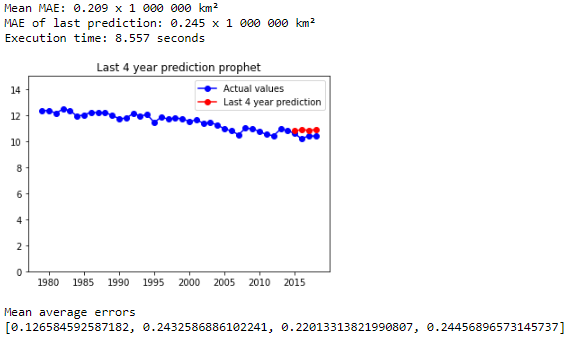
\includegraphics[width=1\linewidth]{uv_ns_prophet}
\end{figure}


\captionof{listing}{Finale iteratie Prophet}
\begin{minted}[
frame=lines,
framesep=2mm,
fontsize=\footnotesize,
linenos,breaklines
]{python}

%%time

# Disabled tf warning because of clutter
warnings.filterwarnings("ignore") # specify to ignore warning messages

start_time = timeit.default_timer()

# initialize variables
maes = []

for train_index, test_index in tscv.split(ts_formated_prophet):
    if train_index.size > 20:  
    
        # initialize cross validation train and test sets
        train  = ts_formated_prophet.iloc[train_index]
        y_test = ts_formated_prophet.iloc[test_index][['y']].values.flatten()
        X_test = ts_formated_prophet.iloc[test_index][['ds']]
        
        # build model
        model = Prophet(**best_params, weekly_seasonality=False, daily_seasonality=False)
        model.fit(train)
        
        # make predictions
        forecast = model.predict(X_test)
        y_pred = forecast['yhat'].values
        
        # error calc
        maes.append(mean_absolute_error(y_test, y_pred))
        
        # last actual prediction 
        last_prediction_prophet = y_pred


# store results
time_Prophet = timeit.default_timer() - start_time
MAE_Prophet = np.mean(maes)
last_MAE_Prophet = maes[-1]

# visualize results
print()
print('Mean MAE: %.3f x 1 000 000 km\u00b2' % MAE_Prophet)
print('MAE of last prediction: %.3f x 1 000 000 km\u00b2' % last_MAE_Prophet)
print('Execution time: %.3f seconds' % time_Prophet)
full_graph(last_prediction_prophet, "Last 4 year prediction prophet")
print('Mean average errors')
print(maes)

\end{minted}

\clearpage
\subsection{Evaluatie}

Wanneer deze resultaten gecombineerd worden wordt de tabel die zichtbaar is op figuur \ref{fig:uvnsresult} verkregen. Om dit resultaat grafisch te schetsen worden op figuur\ref{fig:uvnsresultgraph} de laatste voorspellingen voor elk modeltype weergegeven.

Hieruit kunnen dus geconcludeerd worden dat ARIMA het beste gemiddelde resultaat zal halen bij cross validation aangezien het hier een fout van 0.171 x 1 000 000 km\textsuperscript{2} behaalt. Ook de uitvoeringstijd is het laagst bij ARIMA namelijk 0.360 seconden. Dit is een beter dan LSTM met een fout van 0.200 x 1 000 000 km\textsuperscript{2} en een uitvoeringstijd van 5.480 seconden. De voorspelling van Prophet is nog een pak minder accuraat met een fout van 0.252 x 1 000 000 km\textsuperscript{2} en een uitvoeringstijd van 8.891 seconden.


\begin{figure}
    \centering
    \caption{Resultaat van de univariate non-seasonal analyse}
    \label{fig:uvnsresult}
    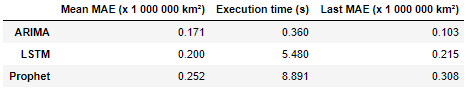
\includegraphics[width=0.7\linewidth]{uv_ns_result}
\end{figure}

\begin{figure}
    \centering
    \caption{Grafische weergave van de laatste voorspellingen van de univariate non-seasonal analyse}
    \label{fig:uvnsresultgraph}
    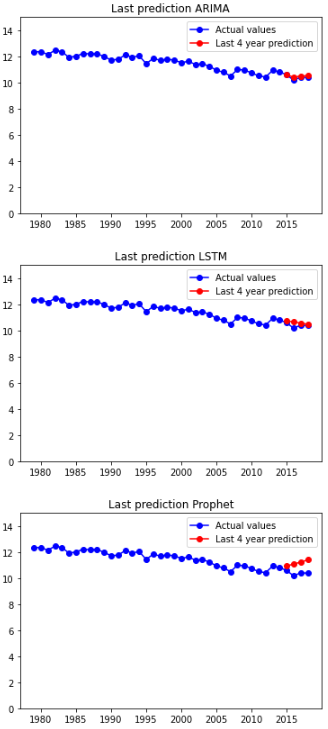
\includegraphics[width=0.7\linewidth]{uv_ns_result_graph}
\end{figure}



\captionof{listing}{Code voor het weergeven van de resultaten}
\begin{minted}[
frame=lines,
framesep=2mm,
fontsize=\footnotesize,
linenos,breaklines
]{python}
# formatting
results = [[MAE_ARIMA,time_ARIMA,last_MAE_ARIMA],[MAE_LSTM,time_LSTM,last_MAE_LSTM],[MAE_Prophet,time_Prophet,last_MAE_Prophet]]

# display results
pd.DataFrame(results, columns=['Mean MAE (x 1 000 000 km\u00b2)','Execution time (s)','Last MAE (x 1 000 000 km\u00b2)'],index=['ARIMA','LSTM','Prophet']).round(decimals=3)

\end{minted}

\captionof{listing}{Code voor het grafisch weergeven van de resultaten}
\begin{minted}[
frame=lines,
framesep=2mm,
fontsize=\footnotesize,
linenos,breaklines
]{python}
# visualize results of last prediction
full_graph(last_prediction_ARIMA, "Last prediction ARIMA")
full_graph(last_prediction_LSTM, "Last prediction LSTM")
full_graph(last_prediction_prophet, "Last prediction Prophet")
\end{minted}

\clearpage

\section{Univariate seizoensgebonden}

In deze sectie zal onderzocht worden welk type model de beste voorspellingen zal treffen voor data met 1 variabele waar er een duidelijk seizoensverband zichtbaar is. Ook hier zal crossvalidation gebruikt worden maar het aantal minimum waarden in de trainingsset zal hier niet 20 zijn maar 300.

\subsection{Algemene methodes}

Vooraleer de dataset effectief gebruikt zal worden dienen er eerst nog enkele functies gedeclareerd te worden.

Zo herkennen kunnen de test\textunderscore stationarity, full\textunderscore graph en  revert\textunderscore diff methodes van de voorgaande sectie herkend worden. Naast deze methodes wordt hier ook nog de revert\textunderscore seasonal\textunderscore diff\textunderscore recursion methode gedefinieerd. Deze wordt benut bij de seizoensgebonden variant van de revert\textunderscore diff methode namelijk revert\textunderscore seasonal\textunderscore diff. Ook deze methode zal dienen om een gedifferentieerde data terug om te zetten naar data die vergeleken kan worden met de effectieve waarden.


\captionof{listing}{Algemene methodes}
\begin{minted}[
frame=lines,
framesep=2mm,
fontsize=\footnotesize,
linenos,breaklines
]{python}
def test_stationarity(timeseries):

    #Determing rolling statistics
    rolmean = timeseries.rolling(36).mean()
    rolstd = timeseries.rolling(24).std()
    
    #Plot rolling statistics:
    orig = plt.plot(timeseries, color='blue',label='Original')
    mean = plt.plot(rolmean, color='red', label='Rolling Mean')
    std = plt.plot(rolstd, color='black', label = 'Rolling Std')
    plt.legend(loc='best')
    plt.title('Rolling Mean & Standard Deviation')
    plt.show(block=False)

def full_graph(predicted, og_dataset, title):
    zerosArray = np.zeros(og_dataset.values.size-len(predicted.flatten()))
    cleanPrediction = pd.Series(np.concatenate((zerosArray,predicted))).replace(0,np.NaN)
    
    # plot
    plt.title(title)
    plt.plot(og_dataset.index, og_dataset.values,marker='o', color='blue',label='Actual values')
    plt.plot(og_dataset.index, cleanPrediction,marker='o', color='red',label='Last 2 year prediction')
    plt.ylim([0,20])
    plt.legend()
    
    plt.show()

def revert_diff(predicted_diff, og_data):
    last_value = og_data.iloc[-predicted_diff.size-1][0]
    predicted_actual = np.array([])
    for value_diff in predicted_diff:
    actual_value = last_value + value_diff
    predicted_actual = np.append(predicted_actual, actual_value)
    last_value = actual_value
    return predicted_actual

def revert_seasonal_diff_recursion(last_seasons_value, diff_value):
    return last_seasons_value + diff_value

def revert_diff_seasonal(predicted_diff, og_data):
    prediction_size = predicted_diff.size

    history = ts[:-prediction_size].values.flatten()
    for value_diff in predicted_diff[-prediction_size:]:
        new_value = revert_seasonal_diff_recursion(history[-12], value_diff)
        history = np.append(history,new_value)
    return history[-prediction_size:]
\end{minted}

\subsection{Stationariteit}

Ook wanneer we hier de stationariteit van de data gaan testen krijgen we een licht dalende trend. Deze trend die zichtbaar is op figuur \ref{fig:uvsstationarity}. Deze loopt gelijk met de trend van de niet seizoensgebonden data aangezien die data het jaarlijks gemiddelde is en dit maandelijkse waarden zijn.

\begin{figure}
    \centering
    \caption{Stationariteit van de originele univariate seizoensgebonden data}
    \label{fig:uvsstationarity}
    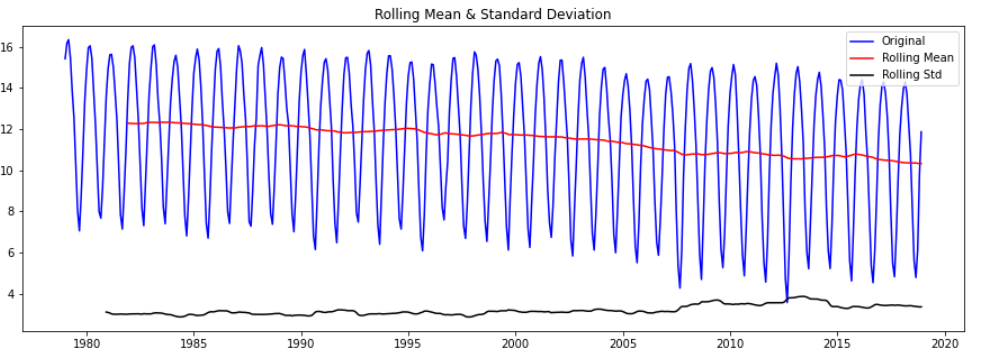
\includegraphics[width=1\linewidth]{uvsstationarity}
\end{figure}

Aangezien hier met seizoensgebonden data gewerkt wordt is het hier naast random walk differentiatie een optie om seizoensdifferentiatie te gebruiken. Dit zal dan ook getest worden. 

\captionof{listing}{Code voor seizoensdifferentiatie}
\begin{minted}[
frame=lines,
framesep=2mm,
fontsize=\footnotesize,
linenos,breaklines
]{python}
ts_diff_seasonal = ts - ts.shift(12)
ts_diff_seasonal = ts_diff_seasonal.dropna()
test_stationarity(ts_diff_seasonal)
\end{minted}

Wanneer seizoensdifferentiatie toegepast wordt zal de stationariteit voorgesteld kunnen worden zoals zichtbaar op figuur\ref{fig:uvsstationarityseasonal}. Dit is wel stationair maar fluctureert wel behoorlijk naar het einde toe.

\begin{figure}
    \centering
    \caption{Stationariteit van de data na seizoensdifferentiatie}
    \label{fig:uvsstationarityseasonal}
    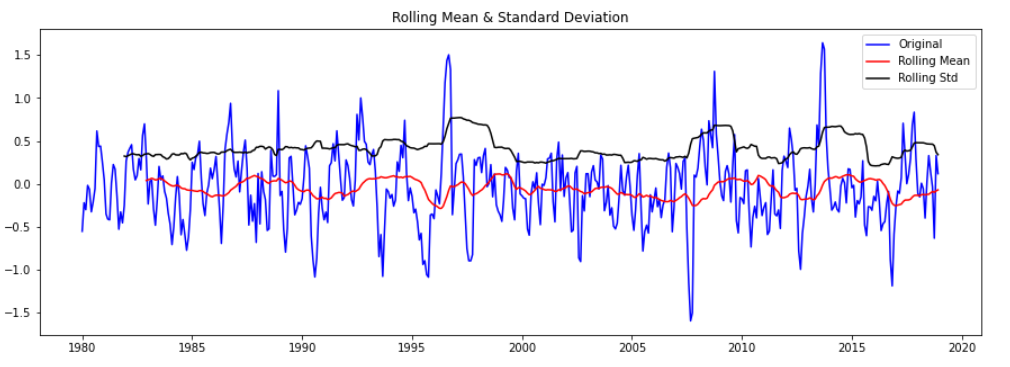
\includegraphics[width=1\linewidth]{uvsstationarityseasonal}
\end{figure}

Daarnaast kan ook nog gewone random walk differentiatie toegepast worden op de data. De stationariteit van deze gedifferentieerde data wordt afgebeeld op figuur\ref{fig:uvsstationarityrw}. Hier wordt vastgesteld dat het gemiddelde een horizontale lijn is. Dit houdt in dat de data zeer stationair is.

\begin{figure}
    \centering
    \caption{Stationariteit van de data na random walk differentiatie}
    \label{fig:uvsstationarityrw}
    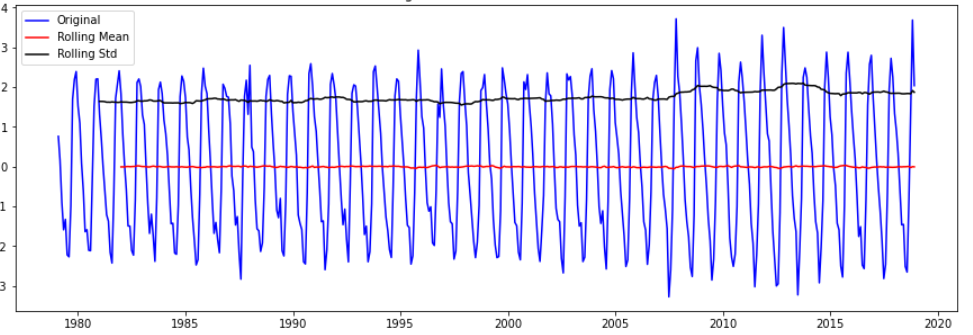
\includegraphics[width=1\linewidth]{uvsstationarityrw}
\end{figure}


\captionof{listing}{code voor differentiatie}
\begin{minted}[
frame=lines,
framesep=2mm,
fontsize=\footnotesize,
linenos,breaklines
]{python}
ts_diff = ts - ts.shift(1)
ts_diff = ts_diff.dropna()
test_stationarity(ts_diff)
\end{minted}

Er dient ook nog vermeld te worden dat door 2 verschillende types differentiaties te testen, het aantal gebruikte testsets bij crossvalidation wel verschillen. Zo zullen er bij seizoensdifferentiatie minder waarden beschikbaar zullen zijn. Concreet leidt dit ertoe dat er bij random walk differentiatie 7 trainingssets zijn die meer dan 300 waarden bevatten terwijl er bij seizoensdifferentiatie 6 trainingssets zullen zijn die meer dan 300 waarden bevatten.

\subsection{ARIMA}

Ook hier zal een ARIMA model opgesteld worden zowel voor de random walk gedifferentieerde data als de seizoensgedifferentieerde data.
\subsubsection{Random walk differentiatie}

Ook hier zal aan hyperparameterbepaling gedaan worden. Aangezien zo goed als alles identiek is als bij univariate non-seasonal differentiatie zal de code hiervan niet meer weergegeven worden alle code is echter terug te vinden in de bijlage.

Uit die hyperparameterbepaling zal blijken dat de combinatie (3,0,4) de beste prestatie zal leveren wanneer het bereik van de parameters $p$ en $q$ 5 zal zijn. 

Wanneer deze hyperparameters ingevoerd worden wordt het resultaat dat afgebeeld staat op figuur \ref{fig:uvsarimadiff} verkregen.

\begin{figure}
    \centering
    \caption{Resultaat van ARIMA bij random walk differentiatie}
    \label{fig:uvsarimadiff}
    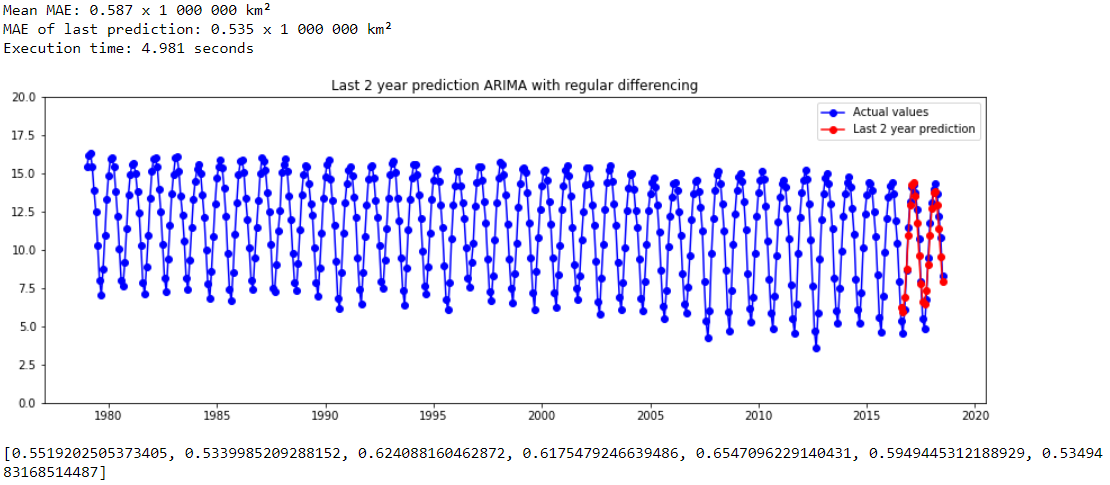
\includegraphics[width=1\linewidth]{uv_s_arima_diff}
\end{figure}


\subsubsection{Seizoensdifferentiatie}

Ook hier zullen eerst de hyperparameters bepaald worden. Met (3,0,3) als optimale waarden bij een range van 0 tot 5 voor de waarden $p$ of $q$. Wanneer deze waarden uitgebreider getest worden resulteert dit in de uitvoer die waar te nemen valt op figuur\ref{fig:uvsarimasdiff}.


\begin{figure}
    \centering
    \caption{Resultaat van ARIMA bij seizoensdifferentiatie}
    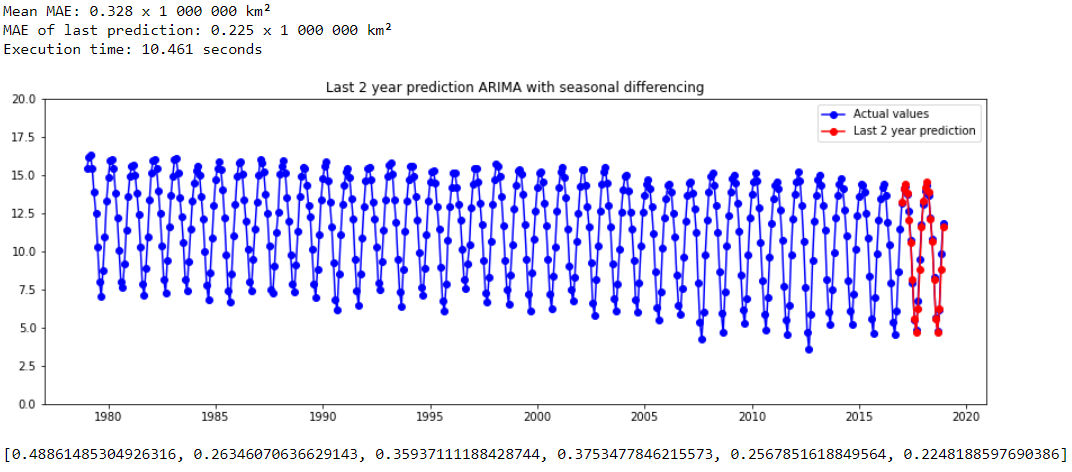
\includegraphics[width=1\linewidth]{uv_s_arima_sdiff}
    \label{fig:uvsarimasdiff}
\end{figure}

\subsection{SARIMA}

Naast ARIMA zelf is er ook een variant op het ARIMA model die specifiek voor data met een seizoenseffect is ontworpen genaamd SARIMA. Deze variant zal in dit deel onder de loep genomen worden.

\subsubsection{Random walk differentiatie} 

De hyperparameterbepaling zal er hier wel anders uitzien, zo dienen voor het seizoenseffect $PDQ$ waarden bepaald te worden naast de $pdq$ waarden voor de data zelf en de $m$ waarde die het aantal tijdstappen zal weergeven van de data die binnen 1 sequentie van het seizoenseffect vallen.

De beste parametercombinatie van de parameters $p, d, q, P, D, Q$ met een bereik van 3 zal (1,0,2,0,1,2) zijn. Het uitgebreid resultaat van deze combinatie wordt weergegeven op figuur\ref{fig:uvssarimaxdiff}.

\begin{figure}
    \centering
    \caption{Resultaat SARIMAX bij random walk differentiatie}
    \label{fig:uvssarimaxdiff}
    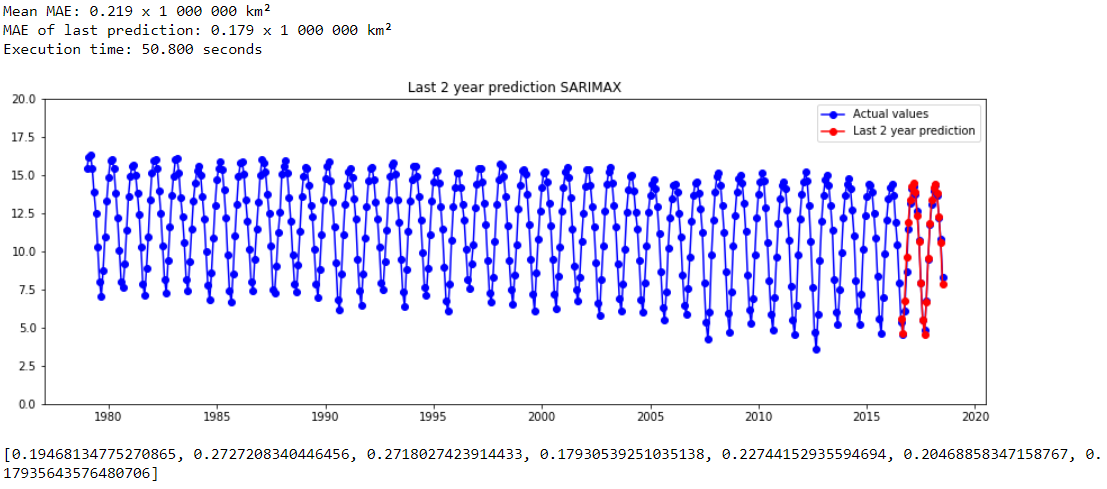
\includegraphics[width=1\linewidth]{uv_s_sarimax_diff}
\end{figure}


\subsubsection{Seizoensdifferentiatie}

Deze testopstelling is identiek aan de vorige uitgezonderd van de invoerdata die hier seizoensgedifferentieerd zal zijn. Ook hier zullen de optimale parameters (1,0,2,0,1,2) zijn. Dit de uitvoer geven die afgebeeld staat op figuur \ref{fig:uvssarimaxsdiff}.

\begin{figure}
    \centering
    \caption{Resultaat SARIMAX bij seizoensdifferentiatie}
    \label{fig:uvssarimaxsdiff}
    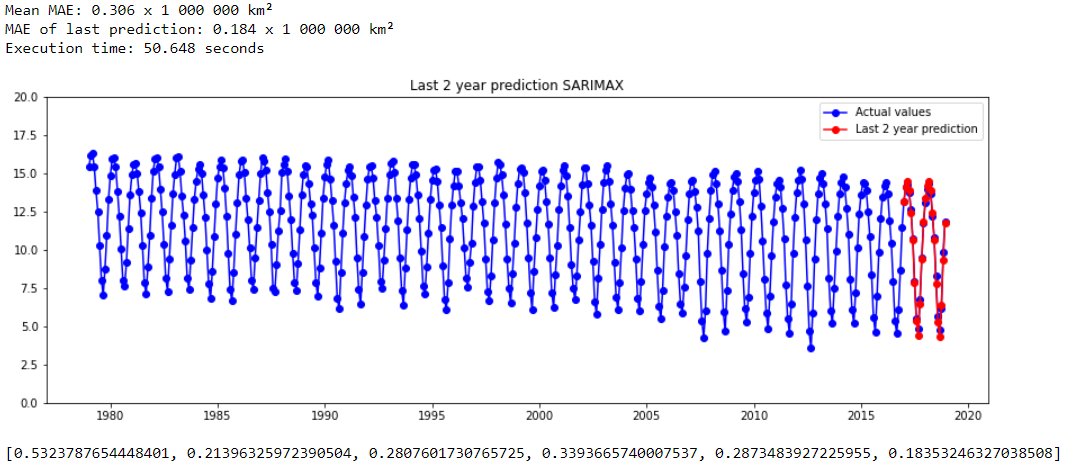
\includegraphics[width=1\linewidth]{uv_s_sarimax_s_diff}
\end{figure}

\subsection{LSTM}
\subsubsection{Random walk differentiatie}

%Ook de opbouw van het LSTM bij seizoensgebonden univariate data verloopt net als die bij niet seizoensgebonden univariate data. Hier bleek er echter wel een verschil in resultaat bij de verschillende hyperparameters en de optimale configuratie met de testwaarden bleek een model te zijn met 1 neuron, waar de dropout rate 0.99 was en een batchgrootte die 8 bedroeg. Het eindresultaat van deze configuratie staat afgebeeld op figuur \ref{fig:uvslstmdiff}.

\subsubsection{Seizoensdifferentiatie}

De opstelling zal identiek zijn als de bovenstaande hier zullen de optimale parameters bestaan uit 1 neuron een dropout rate van 0.99 en een batchgrootte van 8 met het eindresultaat dat zich op figuur \ref{fig:uvslstmsdiff} bevindt.

\begin{figure}
    \centering
    \caption{Resultaat LSTM bij seizoensdifferentiatie}
    \label{fig:uvslstmsdiff}
    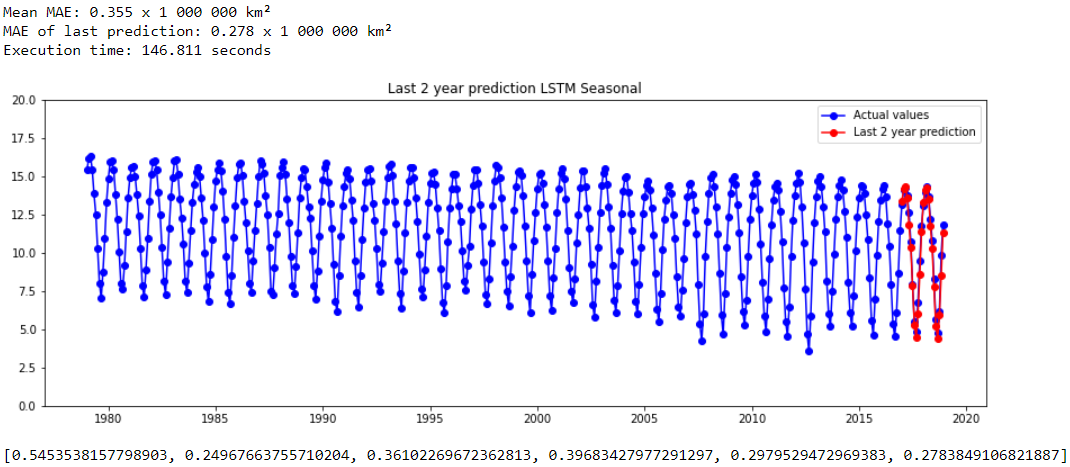
\includegraphics[width=1\linewidth]{uv_s_lstm_s_diff}
\end{figure}

\clearpage
\subsection{Prophet}

Ook hier verloopt alles bijna analoog met de niet seizoensgebonden variatie behalve dat er hier wel 2 hyperparameters getest worden, aangezien er hier wel een seizoenseffect aanwezig is kan de de variabele seasonality\textunderscore prior\textunderscore scale ook onderzocht worden. Het laatste resultaat van de reeks wordt weergegeven op Figuur \ref{fig:uvsprophet}.

\begin{figure}
    \centering
    \caption{Resultaten de voorspellingen voor univariate seizoensgebonden data met Prophet}
    \label{fig:uvsprophet}
    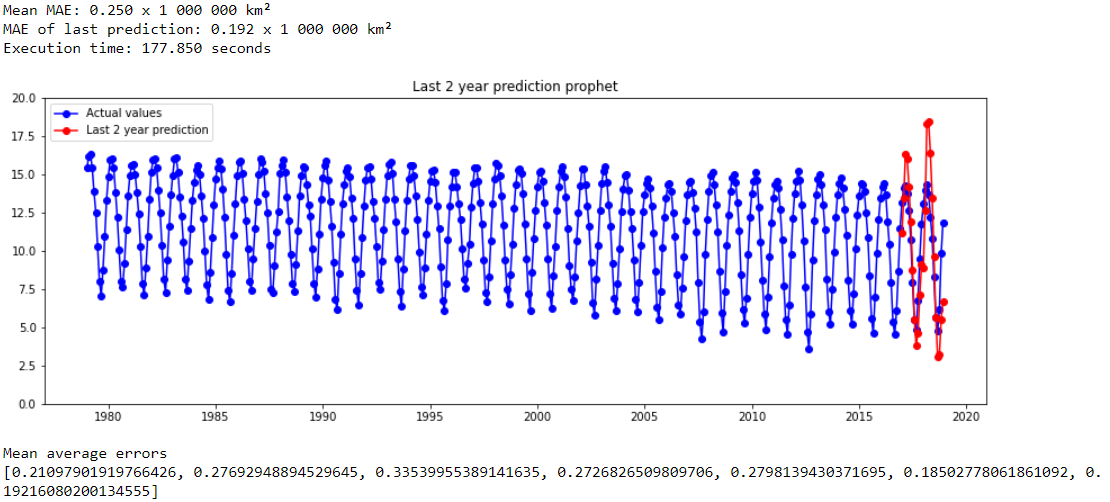
\includegraphics[width=1\linewidth]{uv_s_prophet}
\end{figure}

\clearpage
\subsection{Evaluatie}

Wanneer we de resultaten afgebeeld op Figuur \ref{fig:uv_s_results} beschouwen kunnen we concluderen dat SARIMA met random walk differentiatie de beste voorspellingen zal treffen wanneer we de gemiddelde MAE beschouwen namelijk 0.219 (x 1 000 000 km\textsuperscript{2}). Ook de laatste voorspelling is de meest accurate van alle modellen. Ook de uitvoeringstijd van SARIMA met random walk differencing is relatief laag enkel de ARIMA modellen zijn sneller maar die zijn een stuk minder accuraat.
Het SARIMA-model dat werkt met seizoensgedifferentieerde data presteert een stuk slechter met een gemiddelde MAE van 0.360 (x 1 000 000 km\textsuperscript{2})
\\

Daarnaast presteert het Prophet-model ook goed met een gemiddelde MAE van 0.250 (x 1 000 000 km\textsuperscript{2}) al heeft het wel de op \'{e}\'{e}n na langste uitvoeringstijd. Het ARIMA-model met seizoensdifferentiatie heeft een gemiddelde MAE van 0.328 (x 1 000 000 km\textsuperscript{2}) maar heeft wel de kortste uitvoeringstijd.
De LSTM modellen scoren beide vrij slecht met hoge uitvoeringstijden dus deze vallen niet aan te raden met deze implementatie om seizoensgebonden tijdreeksen te voorspellen.
\\

Bij seizoensgebonden data presteren de LSTM- en ARIMA-modellen beter wanneer er aan seizoensdifferentiatie gedaan wordt, maar de implementatie met random walk differentiatie behaalt de beste score bij SARIMAX dus er kan niet gesteld worden dat de ene soort differentiatie altijd effectiever zal zijn dan de andere. De laatste voorspellingen van alle modeltypes worden weergegeven op Figuren \ref{fig:uvsgraph1} en \ref{fig:uvsgraph2}.


\begin{figure}
    \centering
    \caption{Resultaten van de univariate seizoensgebonden voorspellingen}
    \label{fig:uv_s_results}
    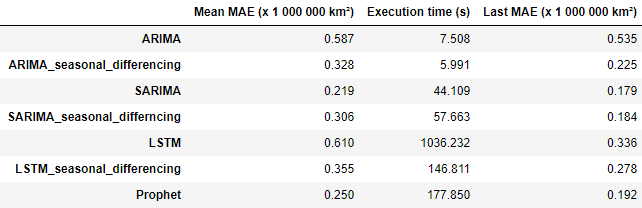
\includegraphics[width=0.9\linewidth]{uv_s_results}
\end{figure}

\begin{figure}
    \centering
    \caption{Grafische weergaven van de laatste voorspellingen van univariate seizoensgebonden data (deel 1)}
    \label{fig:uvsgraph1}
    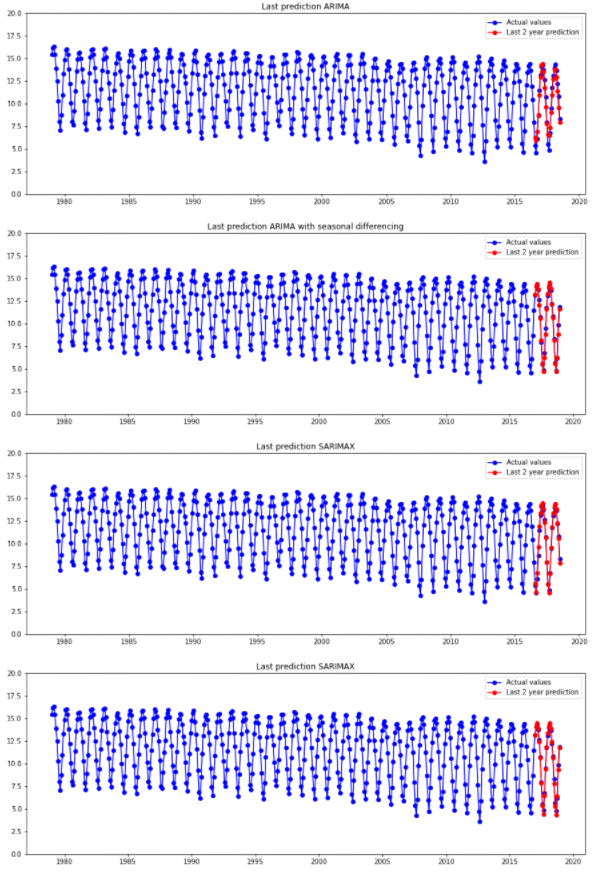
\includegraphics[width=1\linewidth]{uv_s_graph1}
\end{figure}

\begin{figure}
    \centering
    \caption{Grafische weergaven van de laatste voorspellingen van univariate seizoensgebonden data (deel 2)}
    \label{fig:uvsgraph2}
    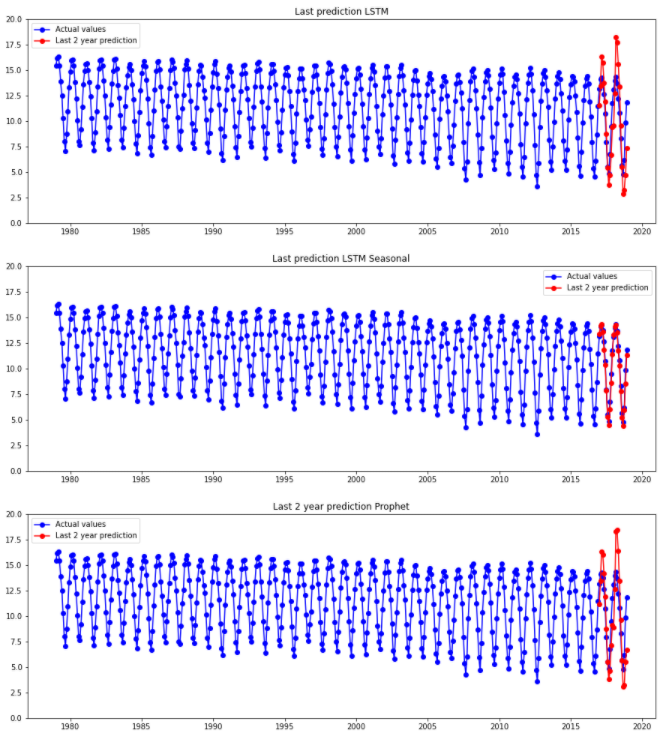
\includegraphics[width=1\linewidth]{uv_s_graph2}
\end{figure}


\section{Multivariate niet-seizoensgebonden}
In dit onderdeel van deze bachelorproef zal onderzocht worden welk van de 3 modellen de beste voorspelling maken voor meervoudige tijdreeksen. Dit houdt in dat het model een tijdreeks krijgt die meerdere features bevat per tijdstap en deze features in verband brengt om tot accuratere voorspellingen te komen. De testset zal dan ook altijd enkel blijven bestaan uit de tijdsstappen die voorspeld moeten worden.

De data die gebruikt zal worden voor deze sectie wordt grafisch weergegeven op Figuur \ref{fig:mvnsdata}. Ook hier zal er gebruik gemaakt worden van cross validation.

Aangezien Prophet geen multivariate tijdreeksen als invoer ondersteunt zal dit niet ge\"{e}valueerd kunnen worden.

\begin{figure}
    \centering
    \caption{Grafische weergave multivariate tijdreeks zonder seizoenseffect}
    \label{fig:mvnsdata}
    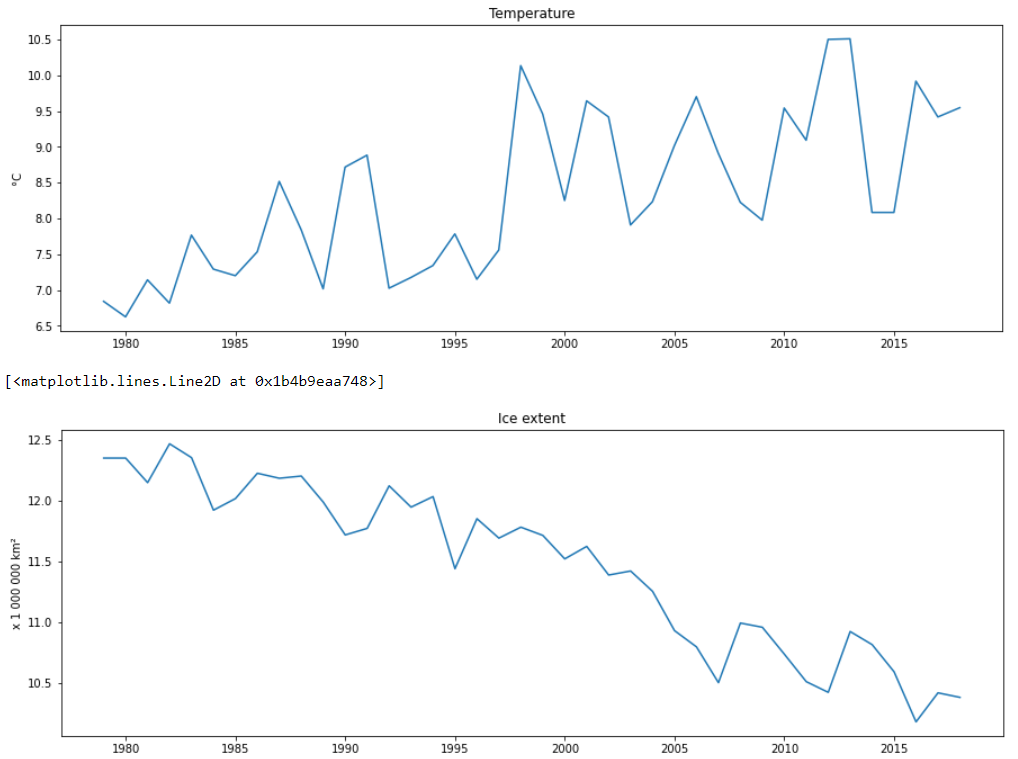
\includegraphics[width=1\linewidth]{mv_ns_data}
\end{figure}

\subsection{Stationariteit}

Ook hier zal de ijsdikte een dalende trend vertonen zoals weergegeven werd bij de univariate analyse en hier zal niks aan veranderen aangezien dit dezelfde data is. Ook deze data zal random walk gedifferentieerd worden maar dit keer niet enkel de ijsdikte maar ook de temperatuur. De resultaten van die differentiatie zijn zichtbaar op figuur \ref{fig:mvnsdatadiff}. Daaruit kan afgeleid worden dat de data nu stationair is.

\begin{figure}
    \centering
    \caption{Grafische weergave gedifferentieerde multivariate tijdreeks zonder seizoenseffect}
    \label{fig:mvnsdatadiff}
    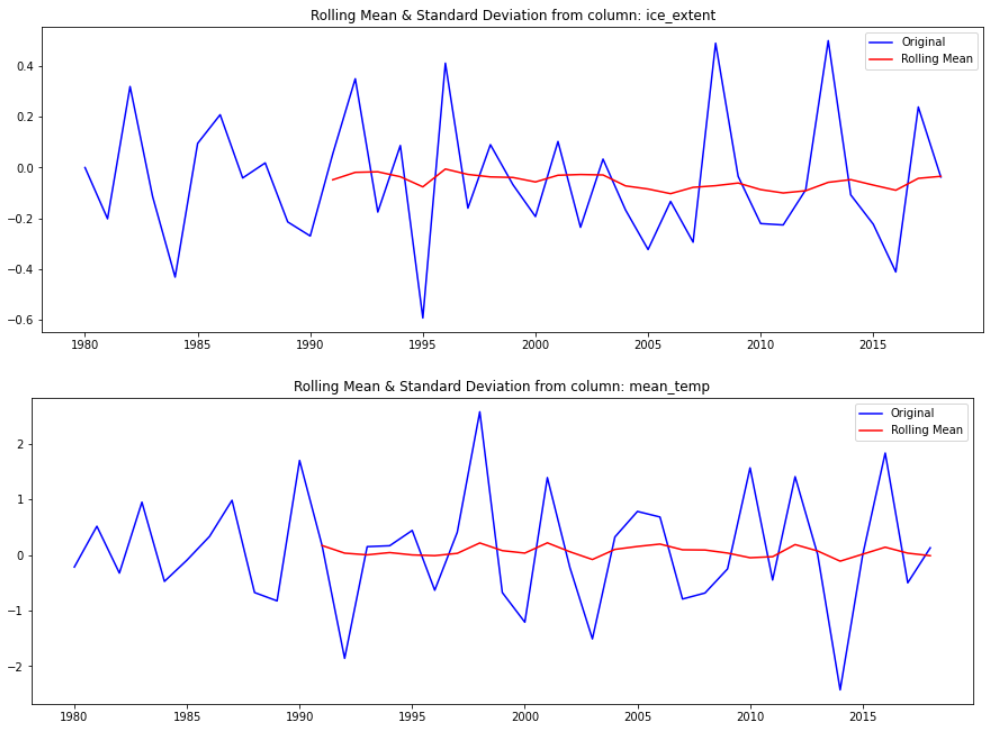
\includegraphics[width=1\linewidth]{mv_ns_data_diff}
\end{figure}

\subsection{VARMAX}
Aangezien een ARIMA model slechts in staat is om tijdreeksen met 1 variabele te voorspellen moet er een variant gebruikt worden die wel in staat is om multivariate tijdreeksen te interpreteren genaamd VARMAX. 

Ook hier wordt de gebruikelijke methode toegepast om de hyperparameters te bepalen en daar verandert niet veel aan. Behalve dat enkel de $p$ en $q$ variabelen verwacht worden, de $d$ variabele is hier niet nodig. 

Bij een range van 0 tot 5 zijn ook hier de optimale waarden voor deze parameters (3,3). Wanneer we deze waarden invoeren in de uitgebreidere versie van de evaluatiemethode wordt het resultaat bekomen dat weergegeven wordt op Figuur \ref{fig:mvnsvarmax}.

\begin{figure}
    \centering
    \caption{Resultaat multivariate voorspelling VARMAX}
    \label{fig:mvnsvarmax}
    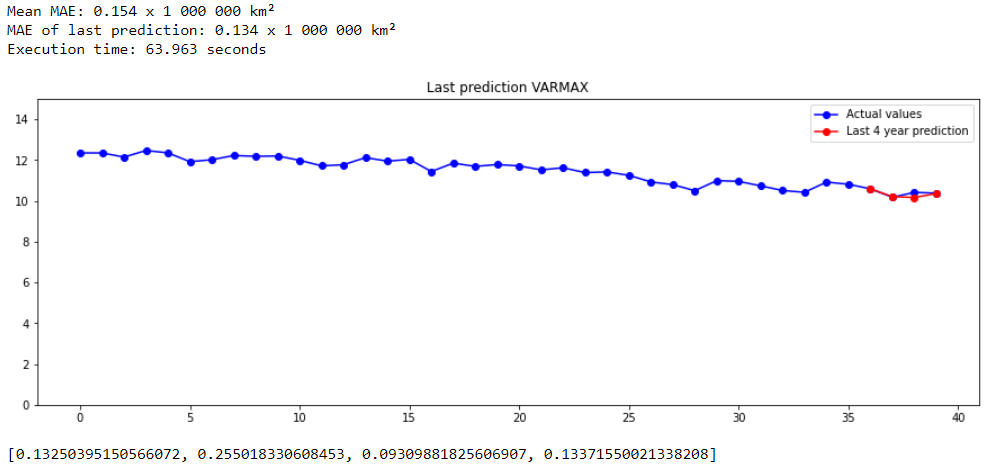
\includegraphics[width=1\linewidth]{mv_ns_varmax}
\end{figure}


\subsection{LSTM}

Waneer er multivariate voorspellingen gemaakt moeten worden met LSTM ziet de structuur van het neuraal netwerk er anders uit dan bij een univariate voorspelling. Zo zal er deze keer een grote functie gebruikt worden om het model op te stellen en de voorspelling te maken. Deze functie staat uitgeschreven bij listing \ref{code:pred_lstm}.

De hyperparameters die hier bepaald zullen worden zijn het aantal neuronen en het aantal epochs om tot het beste resultaat te komen. Een enkel neuron blijkt alweer optimaal te zijn en met 200 epochs verkrijgt men het beste resultaat. De uitgebreide uitvoer van dit resultaat wordt weergegeven op Figuur \ref{fig:mvnslstm}.

\captionof{listing}{Voorspellingsfunctie LSTM}
\label{code:pred_lstm}
\begin{minted}[
frame=lines,
framesep=2mm,
fontsize=\footnotesize,
linenos,breaklines
]{python}
def predict_LSTM(train, test, n_neurons, n_epochs):
    test['sum'] = test['mean_temp'] + test['ice_extent']
    
    
    # define input sequence
    in_seq1 = train.values[:,0]
    in_seq2 = train.values[:,1]
    out_seq = array([in_seq1[i]+in_seq2[i] for i in range(len(in_seq1))])
    
    # convert to [rows, columns] structure
    in_seq1 = in_seq1.reshape((len(in_seq1), 1))
    in_seq2 = in_seq2.reshape((len(in_seq2), 1))
    out_seq = out_seq.reshape((len(out_seq), 1))
    
    # horizontally stack columns
    dataset = hstack((in_seq1, in_seq2, out_seq))
    
    # choose a number of time steps
    n_steps_in, n_steps_out = 4, 4
    
    # covert into input/output
    X, y = split_sequences(dataset, n_steps_in, n_steps_out)
    
    # the dataset knows the number of features, e.g. 2
    n_features = X.shape[2]
    
    # define model
    model = Sequential()
    model.add(LSTM(n_neurons, activation='relu', input_shape=(n_steps_in, n_features)))
    model.add(RepeatVector(n_steps_out))
    model.add(LSTM(n_neurons, activation='relu', return_sequences=True))
    model.add(TimeDistributed(Dense(n_features)))
    model.compile(optimizer='adam', loss='mae')
    
    # fit model
    model.fit(X, y, epochs=n_epochs, verbose=0)
    
    # demonstrate prediction
    x_input = test.values
    x_input = x_input.reshape((1, n_steps_in, n_features))
    yhat = model.predict(x_input, verbose=0)
    return yhat
\end{minted}

\begin{figure}
    \centering
    \caption{Resultaat multivariate voorspelling LSTM}
    \label{fig:mvnslstm}
    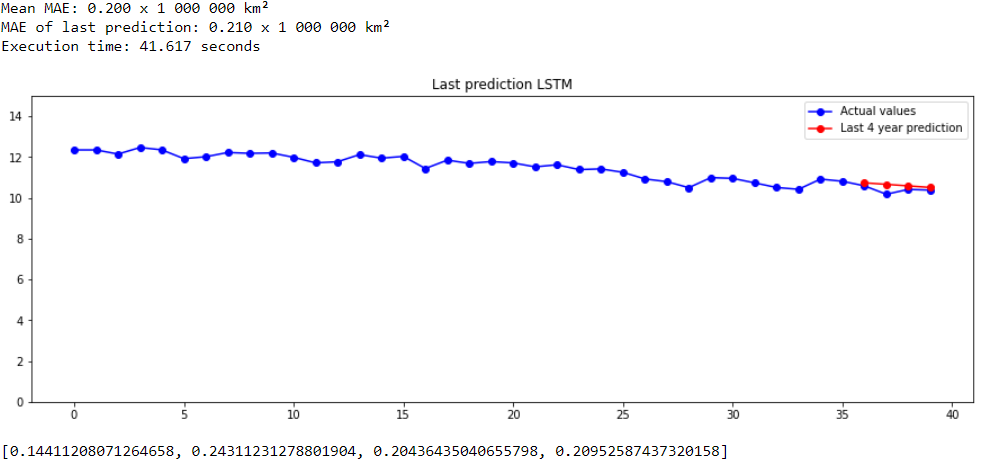
\includegraphics[width=1\linewidth]{mv_ns_LSTM}
\end{figure}
\clearpage

\subsection{Evaluation}

Wanneer we de resultaten van de multivariate niet-seizoensgebonden voorspellingen weergegeven op Figuur \ref{fig:mvnsresult} vergelijken kunnen we stellen dat VARMAX het best presteert volgens cross validation maar wel een hogere uitvoeringstijd heeft. Daarnaast zal de laatste voorspelling van het ijsoppervlak door het VARMAX model ook accurater zijn dan dat van het LSTM model. Deze laatste voorspelling wordt grafisch weergegeven op Figuur \ref{fig:mvnsresultgraph}.

\begin{figure}
    \centering
    \caption{Resultaten multivariate voorspelling}
    \label{fig:mvnsresult}
    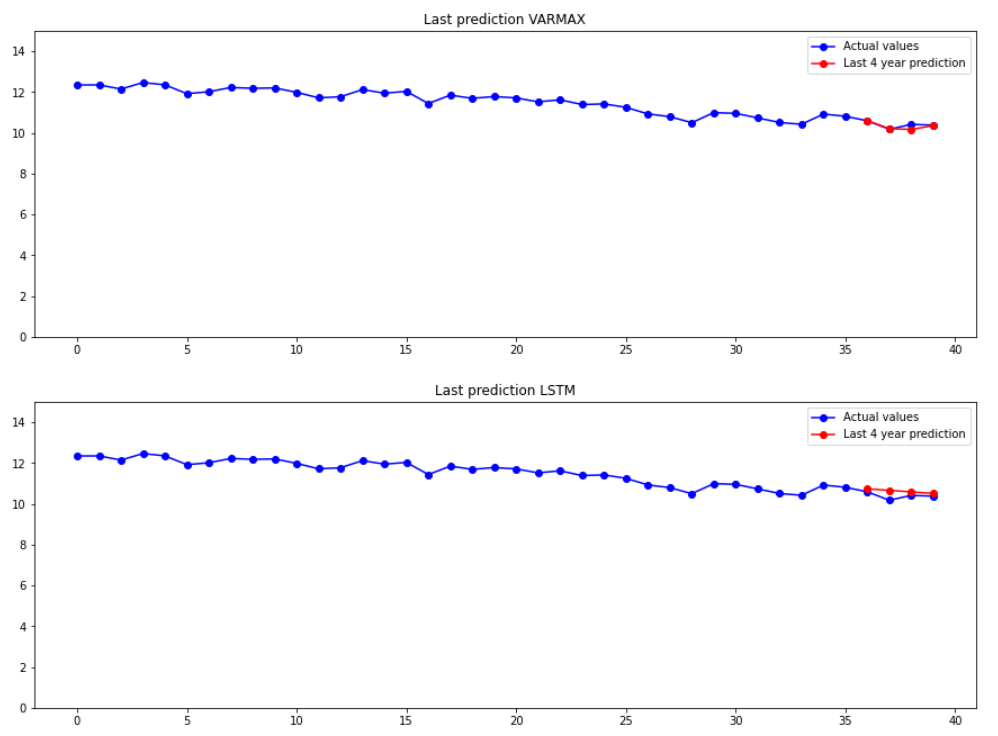
\includegraphics[width=1\linewidth]{mv_ns_result}
\end{figure}

\begin{figure}
    \centering
    \caption{Grafische weergaven van de laatste voorspellingen van de VARMAX en LSTM modellen}
    \label{fig:mvnsresultgraph}
    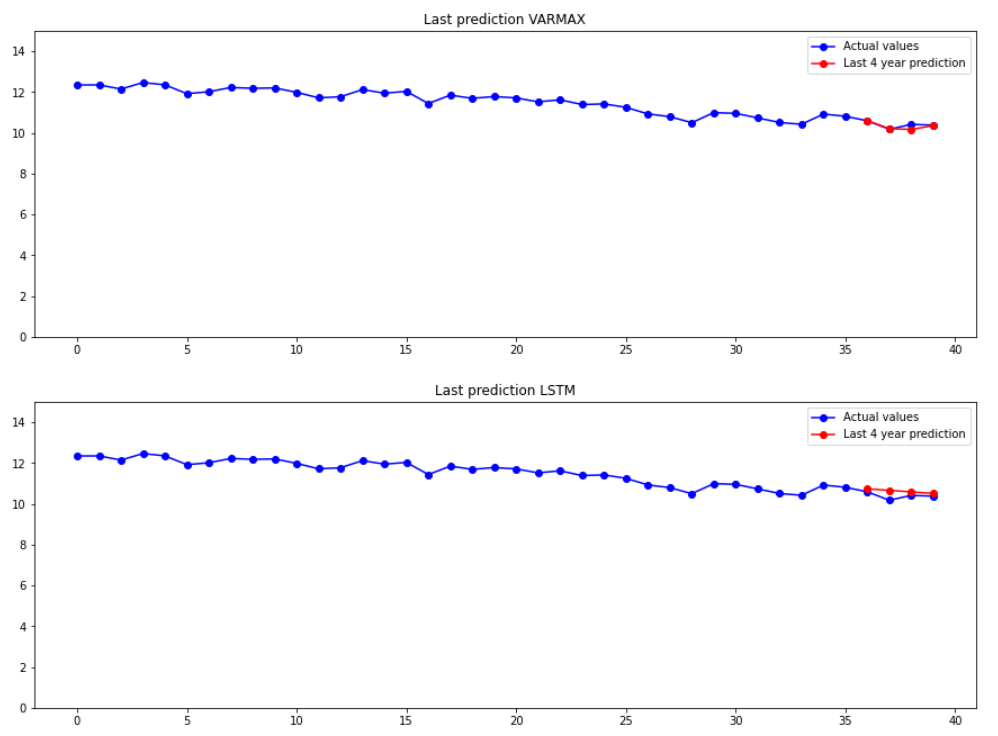
\includegraphics[width=1\linewidth]{mv_ns_result_graph}
\end{figure}



\section{Multivariate seizoensgebonden}

De laatste combinatie die getest zal worden is de dataset waar een seizoensverband en een extra variabele aanwezig is. Deze extra variabele zal andermaal de temperatuur zijn in een dataset die de maandelijkse temperatuur en ijsdikte zal bevatten. Hier zullen ook, net als bij de niet seizoensgebonden data, enkel VARMAX en LSTM getest worden. Hier zal ook weer cross validation gebruikt worden. Er zal ook weer random walk en seasonal differentiatie gebuikt worden.

\subsection{VARMAX}
\subsubsection{Random walk differentiatie}

Waneer we de hyperparameters bepalen bij dit VARMAX model blijken de parameters (4,1) de optimale waarden te zijn bij een range van 0 tot 5. Wanneer we deze invoeren om een uitgebreider resultaat te krijgen bekomen we de uitvoer die te beschouwen valt op Figuur \ref{fig:mvsvarmaxdiff}.

\begin{figure}
    \centering
    \caption{Resultaat VARMAX bij random walk differentiatie}
    \label{fig:mvsvarmaxdiff}
    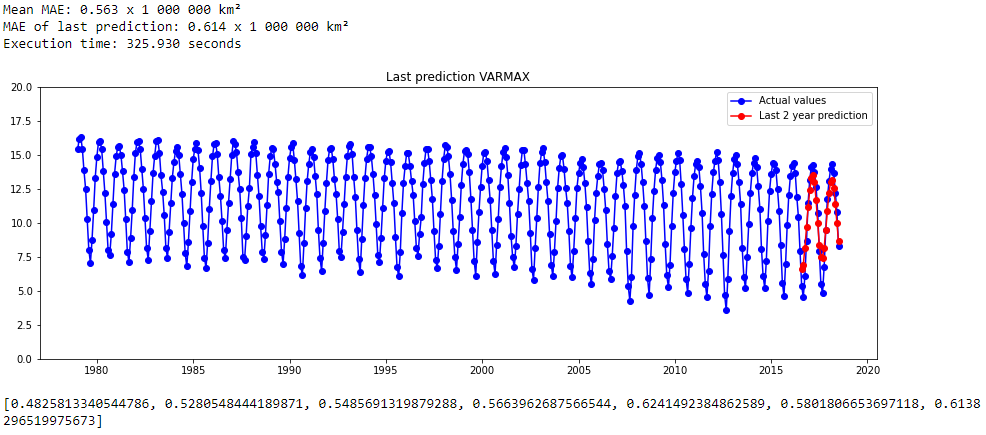
\includegraphics[width=1\linewidth]{mv_s_varmax_diff}
\end{figure}


\subsubsection{Seizoensdifferentiatie}
De optimale hyperparameters bij het VARMAX model dat opgebouwd wordt op basis van seizoensgedifferentieerde data zijn (0,1) wanneer de range van 0 tot 5 loopt. Het resultaat van dit model wordt afgebeeld op Figuur \ref{fig:mvsvarmaxsdiff}.


\begin{figure}
    \centering
    \caption{Resultaat VARMAX bij seizoensdifferentiatie}
    \label{fig:mvsvarmaxsdiff}
    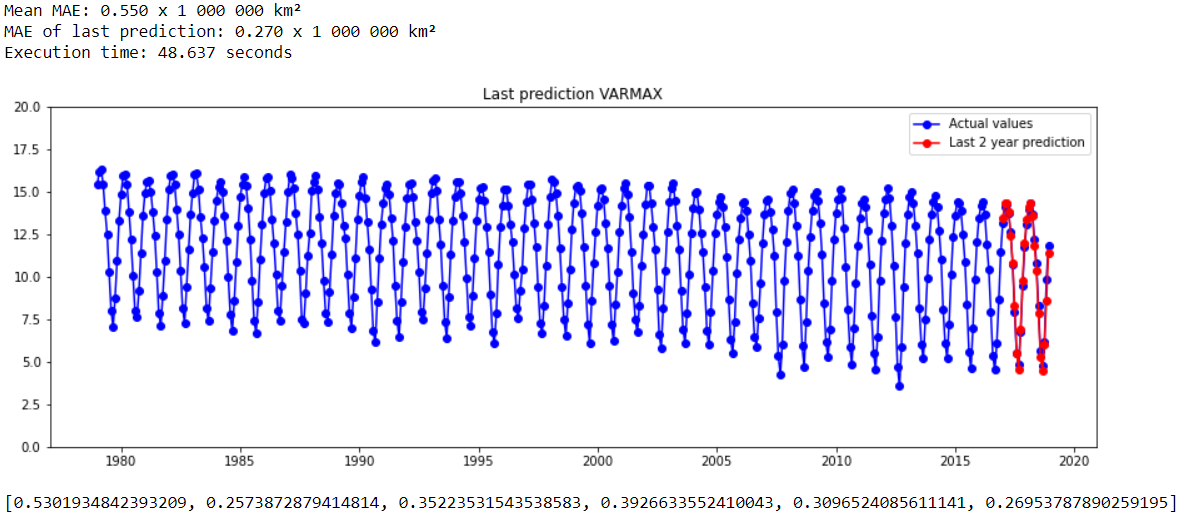
\includegraphics[width=1\linewidth]{mv_s_varmax_s_diff}
\end{figure}


\subsection{LSTM}
\subsubsection{Random walk differentiatie}
De optimale parameters bij Random walk differentiatie en bleken 30 neuronen te zijn en 300 epochs. Een hoger aantal neuronen en epochs zouden leiden tot een beter resultaat aangezien de MAE verlaagde naargelang deze parameters verhoogden maar er moest een grens getrokken worden om de uitvoeringstijd beperkt te houden. Wanneer we het model met de aangegeven parameters analyseren zullen we het resultaat bekomen dat op Figuur \ref{fig:mvslstmdiff}.

\begin{figure}
    \centering
    \caption{Resultaat LSTM bij random walk differentiatie}
    \label{fig:mvslstmdiff}
    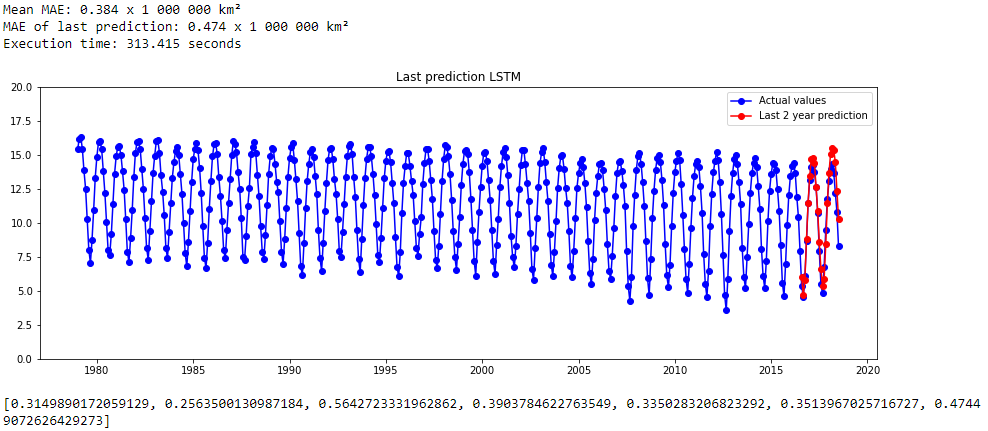
\includegraphics[width=1\linewidth]{mv_s_lstm_diff}
\end{figure}


\subsubsection{Seizoensdifferentiatie}
De parameters die voor het beste resultaat zorgen bij het LSTM-model en seizoensgedifferentieerde data zijn 1 voor het aantal neuronen en 200 voor het aantal epochs en in tegenstelling tot de random walk differentiatie blijkt het verhogen van deze parameters niet te zorgen voor betere resultaten. Het resultaat van dit model wordt afgebeeld op Figuur \ref{fig:mvslstmsdiff}.


\begin{figure}
    \centering
    \caption{Resultaat LSTM seizoensdifferentiatie}
    \label{fig:mvslstmsdiff}
    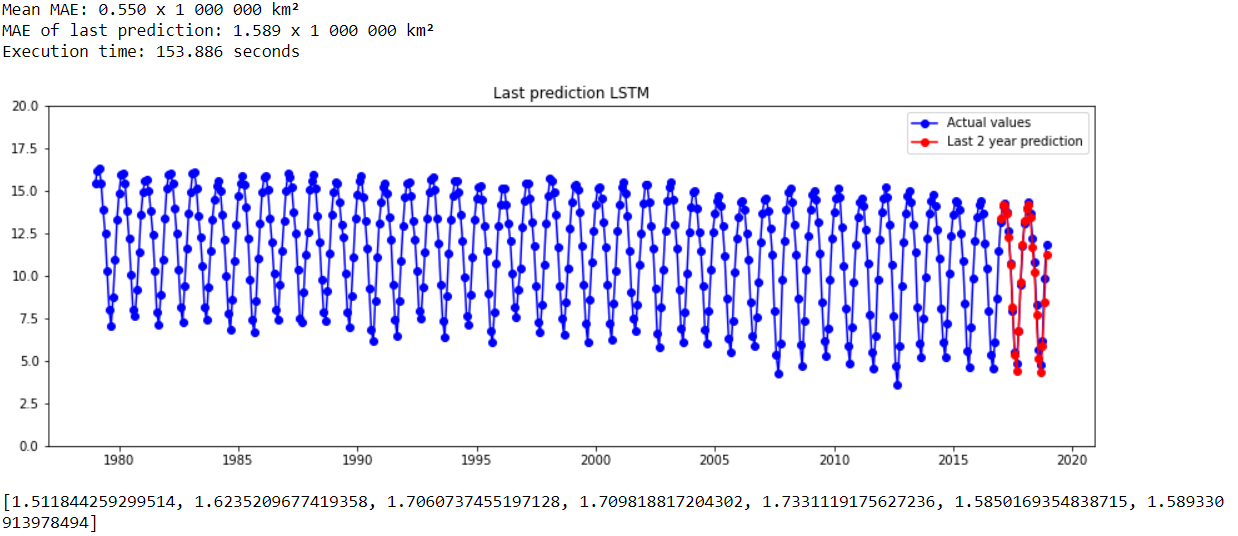
\includegraphics[width=1\linewidth]{mv_s_lstm_s_diff}
\end{figure}

\clearpage

\subsection{Evaluation}
Wanneer we de resultaten op figuur \ref{fig:mvsresults} beschouwen kunnen we duidelijk aflezen dat LSTM met random walk differencing de laagste gemiddelde fout zal hebben en dus het best zal scoren wanneer we ons baseren op cross validation. Het scoort een stuk beter dan de andere modellen die allemaal een zeer gelijkaardige MAE hebben. Dit model zal echter wel de hoogste uitvoeringstijd hebben. \\

Het VARMAX model met seizoensdifferentiatie zal de beste score behalen wanneer we naar de laatste voorspelling kijken en zal ook de laagste uitvoeringstijd hebben dus dit zou op vlak van uitvoeringssnelheid een goed alternatief zijn. De grafische weergaven van de laatste voorspellingen zijn zichtbaar op Figuur \ref{fig:mvsresultsgraphs}. De waarden tussen de modellen die random walk differentiatie gebruiken zullen ietwat verschillen van degene die gebruik maken van seizoensdifferentiatie aangezien de data met 5 tijdstappen getransformeerd moest worden om tot evenwaardige testsetgroottes te komen. Dit was noodzakelijk om alle modellen met elkaar te vergelijken.


\begin{figure}
    \centering
    \caption{Resultaten multivariate seizoensgebonden voorspellingsmodellen}
    \label{fig:mvsresults}
    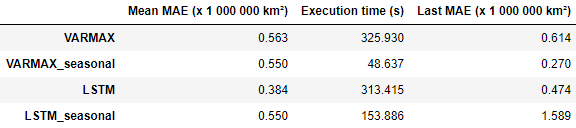
\includegraphics[width=0.8\linewidth]{mv_s_results}
\end{figure}


\begin{figure}
    \centering
    \caption{Grafische weergaven van de laatste voorspellingen van multivariate seizoensgebonden voorspellingsmodellen}
    \label{fig:mvsresultsgraphs}
    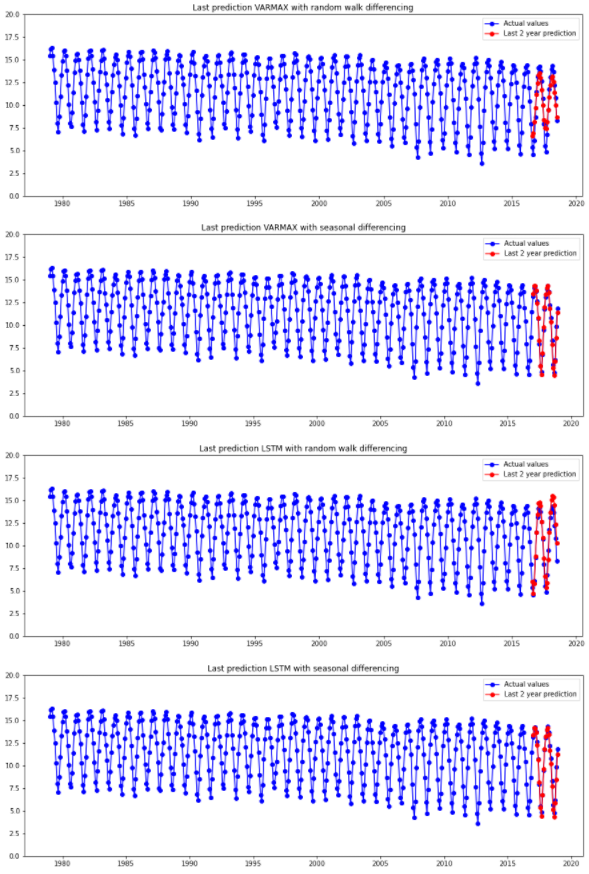
\includegraphics[width=1\linewidth]{mv_s_results_graphs}
\end{figure}

